\documentclass{beamer}
\setbeamertemplate{footline}[frame number]
\usepackage{graphicx}
\usepackage{epstopdf}
\usepackage{caption}
\usepackage{subcaption}
\usepackage{lmodern}
\usepackage{siunitx}
\usepackage[version=3]{mhchem}
\graphicspath{{figures/}}
\newcolumntype{C}{>{\centering\arraybackslash} m{0.1cm} }  %# New column type
\newcolumntype{V}{>{\centering\arraybackslash} m{0.45\linewidth} }
\AtBeginSection{\frame{\sectionpage}}
\AtBeginSubsection{\frame{\subsectionpage}}

\title{High Energy Event Reconstruction}
\subtitle{}
\author[Michinari]{Michinari Sakai}
\institute{University of Hawaii}
\date{2014 September 4}

\begin{document}

\frame{\titlepage}

\section{Energy Calibration}

\begin{frame}
	\frametitle{High Energy ($>\sim$\SI{1}{\giga\electronvolt}) Calibration}
	%\framesubtitle{}
	\begin{itemize}
		\item KamLAND has traditionally used energy calibrations for lower
			energy regimes ($\sim$\SI{}{\mega\electronvolt})
		\item Can this calibration be used for higher energy
			($\sim$\SI{}{\giga\electronvolt}) events too?
		\item Need energy calibration for higher energies
		\item Candidates:\\
			\begin{itemize}
				\item linac
					(\SIrange[range-phrase=--]{5}{10}{\mega\electronvolt})
				\item Michel electron (\SI{\sim50}{\mega\electronvolt})
				\item cosmic ray muon
			\end{itemize}
		\item Choose cosmic ray muon b/c it is the only source with
			\SI{}{\giga\electronvolt} range
			energies
	\end{itemize}
\end{frame}

\begin{frame}
	\frametitle{Muon candidate selection}
	For each run, choose
	\begin{itemize}
		\item 1000 LS muons (impact parameter $<$ \SI{650}{\centi\meter})
		\item 1000 MO muons (impact parameter $>$ \SI{650}{\centi\meter})
	\end{itemize}
	\begin{columns}[t]
		\column{0.5\textwidth}
		MO muons (run 5000)
		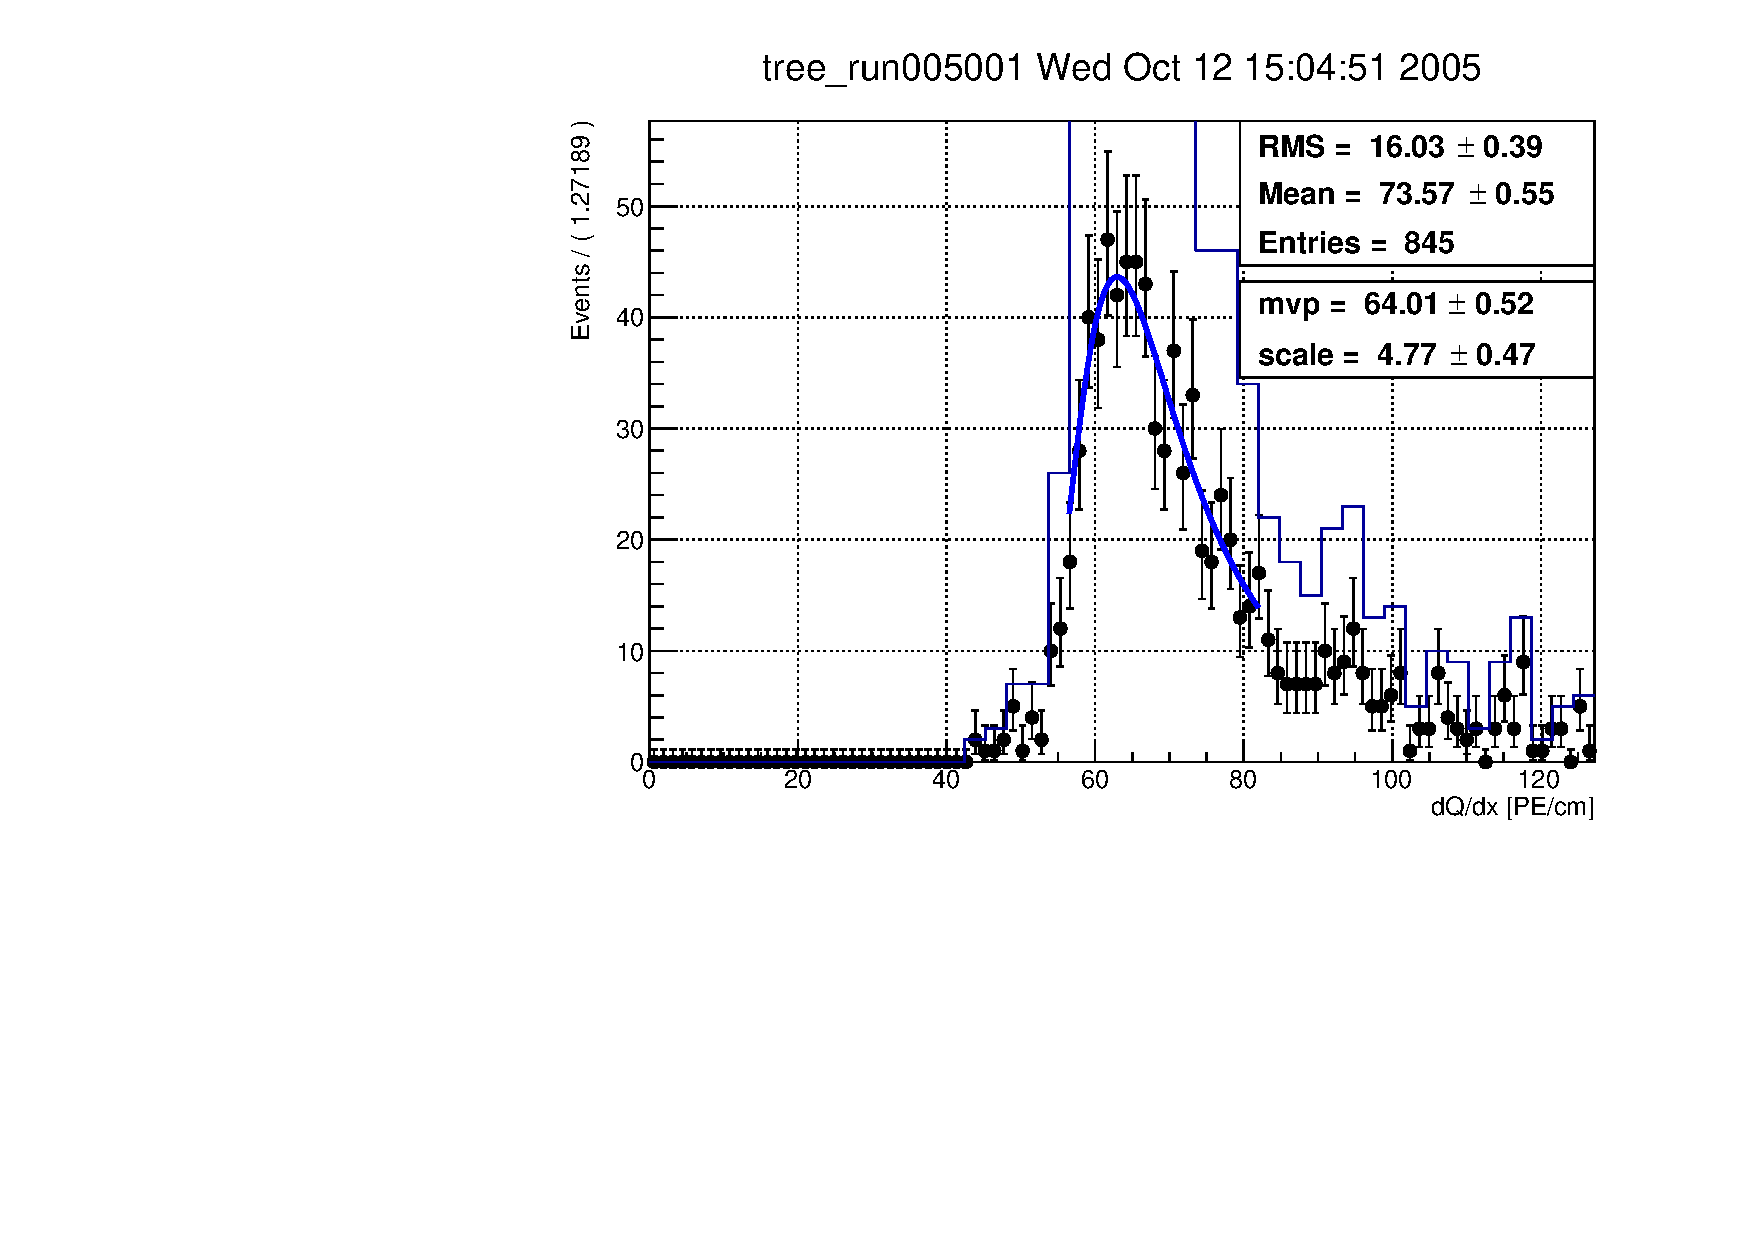
\includegraphics[width=\textwidth]{tree_run005001_cherenID_dQdx.pdf}
		\column{0.5\textwidth}
		LS muons (run 5000)
		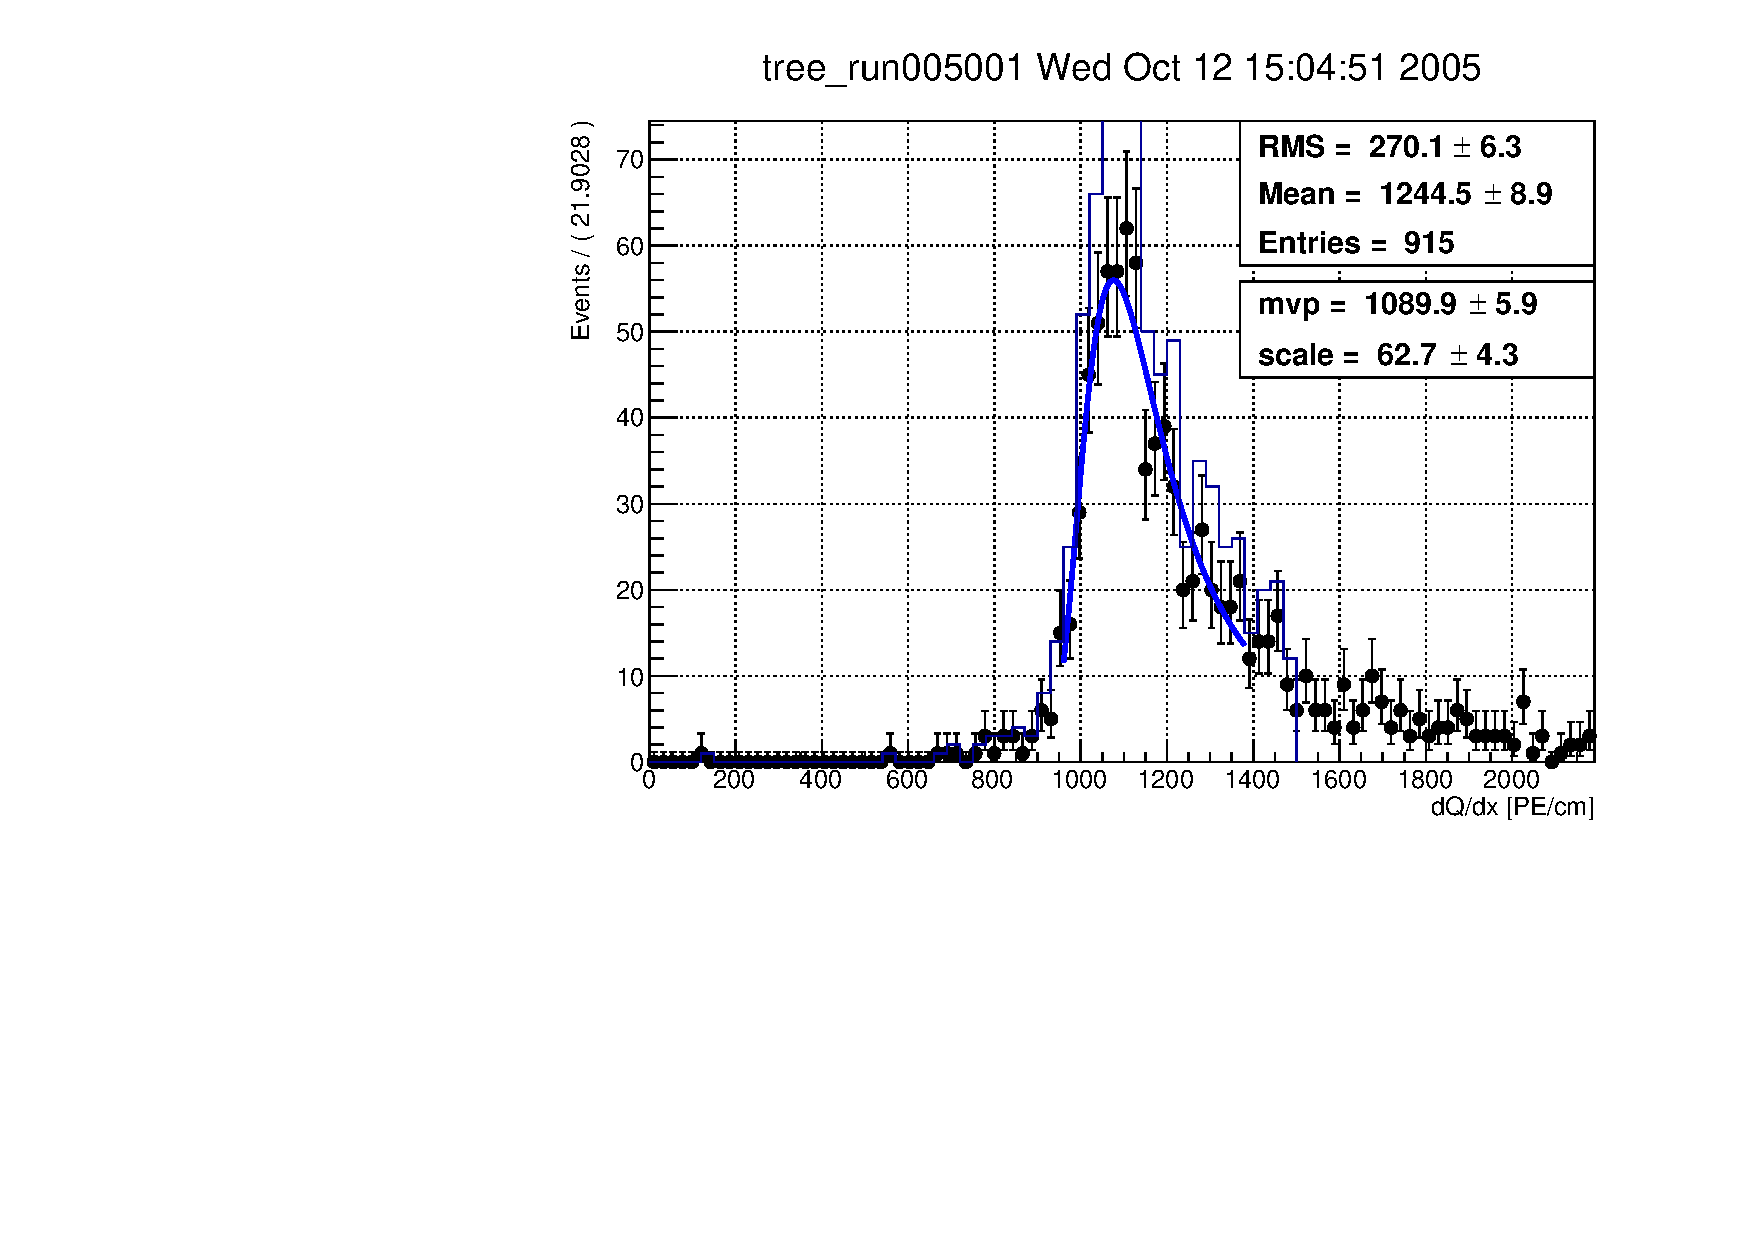
\includegraphics[width=\textwidth]{tree_run005001_scintID_dQdx.pdf}

	\end{columns}
	Subtract Cherenkov component to get scintillation component of LS muons
\end{frame}

\begin{frame}
	\frametitle{Convert dx $\to$ dE using muon events in LS (KLG4)}
	\begin{figure}
		\centering
		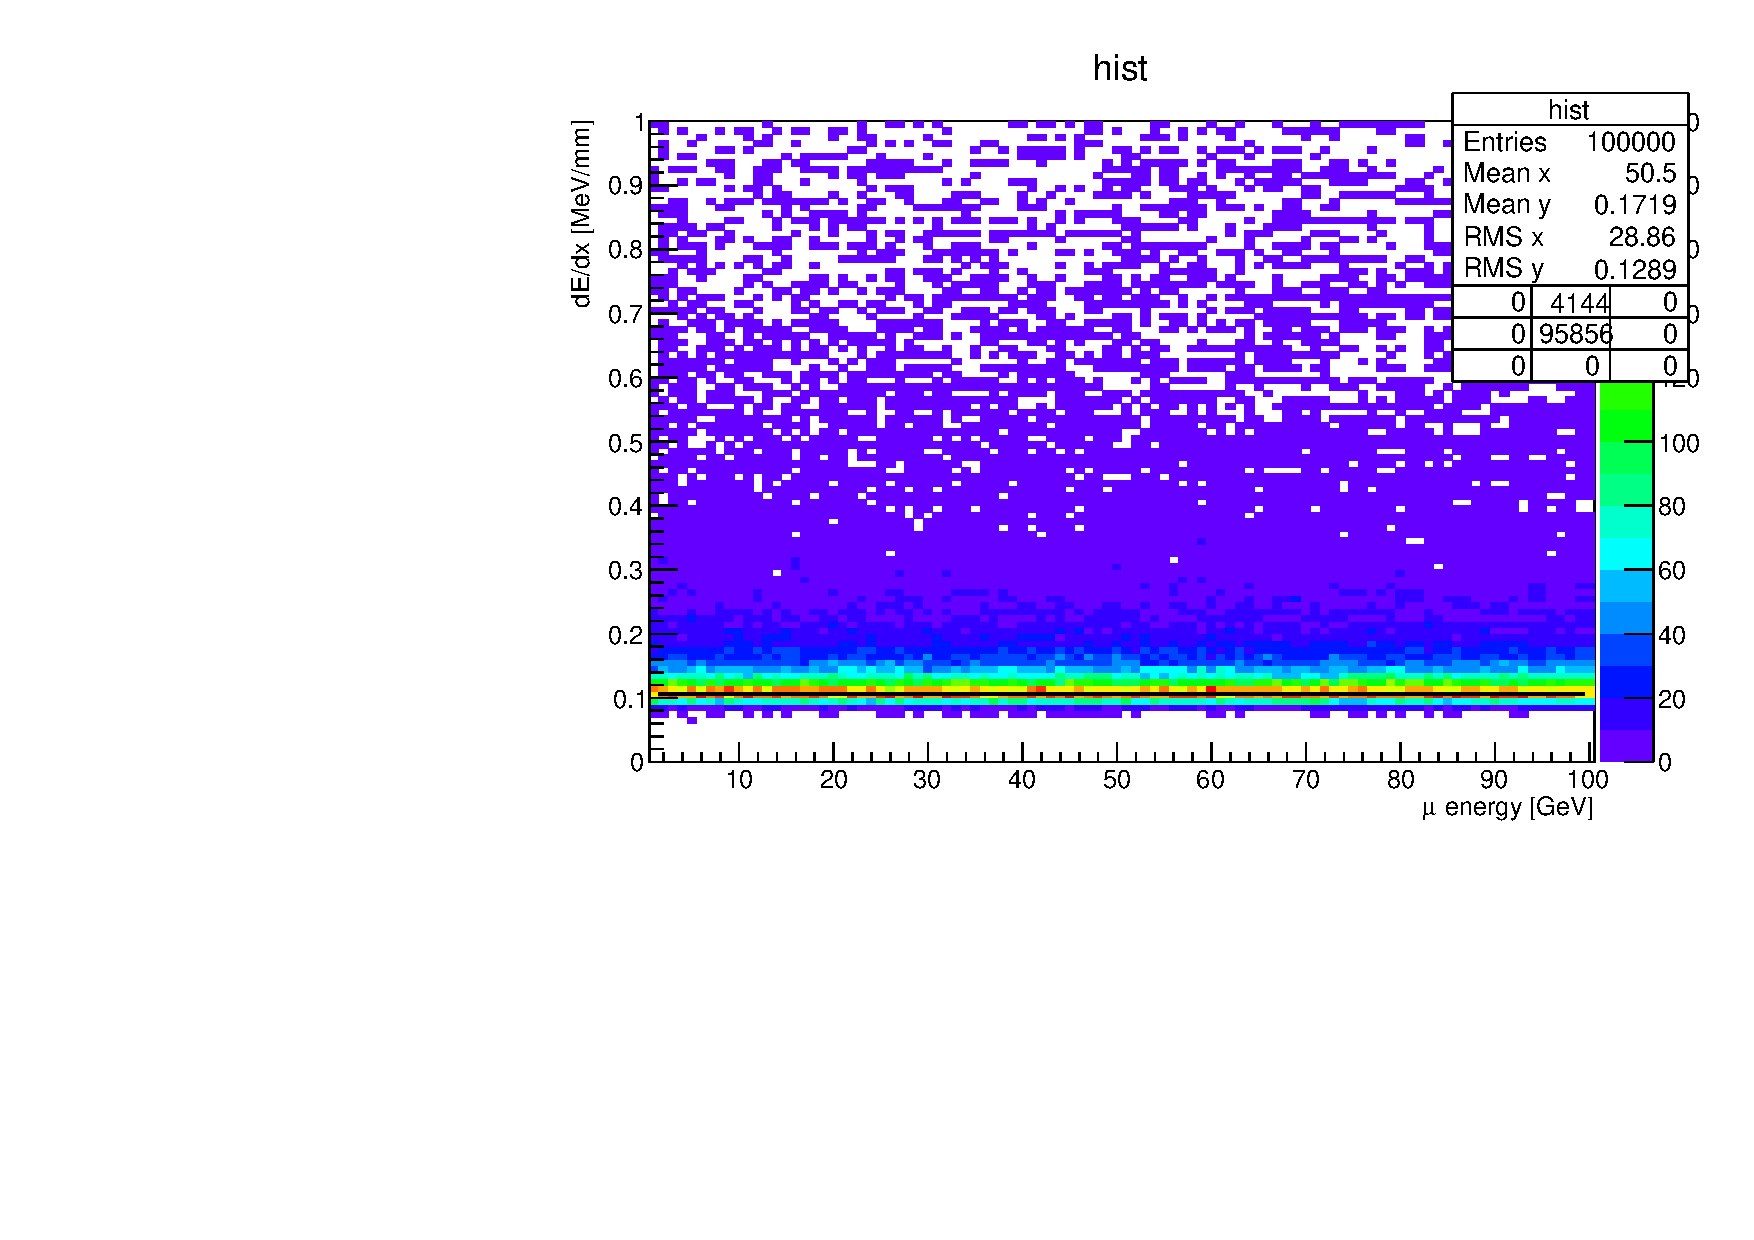
\includegraphics[width=\textwidth]{muStoppingPower_1to100GeV.pdf}
		\caption{
			Use average value of dE/dx =
			\SI{1.719}{\mega\electronvolt\per\centi\meter}
		}
	\end{figure}
\end{frame}

\begin{frame}
	\frametitle{PE/MeV for all runs (new high-energy calibration)}
	\begin{tabular}{|C|V|V|}
		\hline
		&TotalCharge17 &TotalChargeID \\
		\hline
		\rotatebox[origin=c]{90}{$\text{PE}_{\text{scint}}/\SI{}{\mega\electronvolt}$} &
		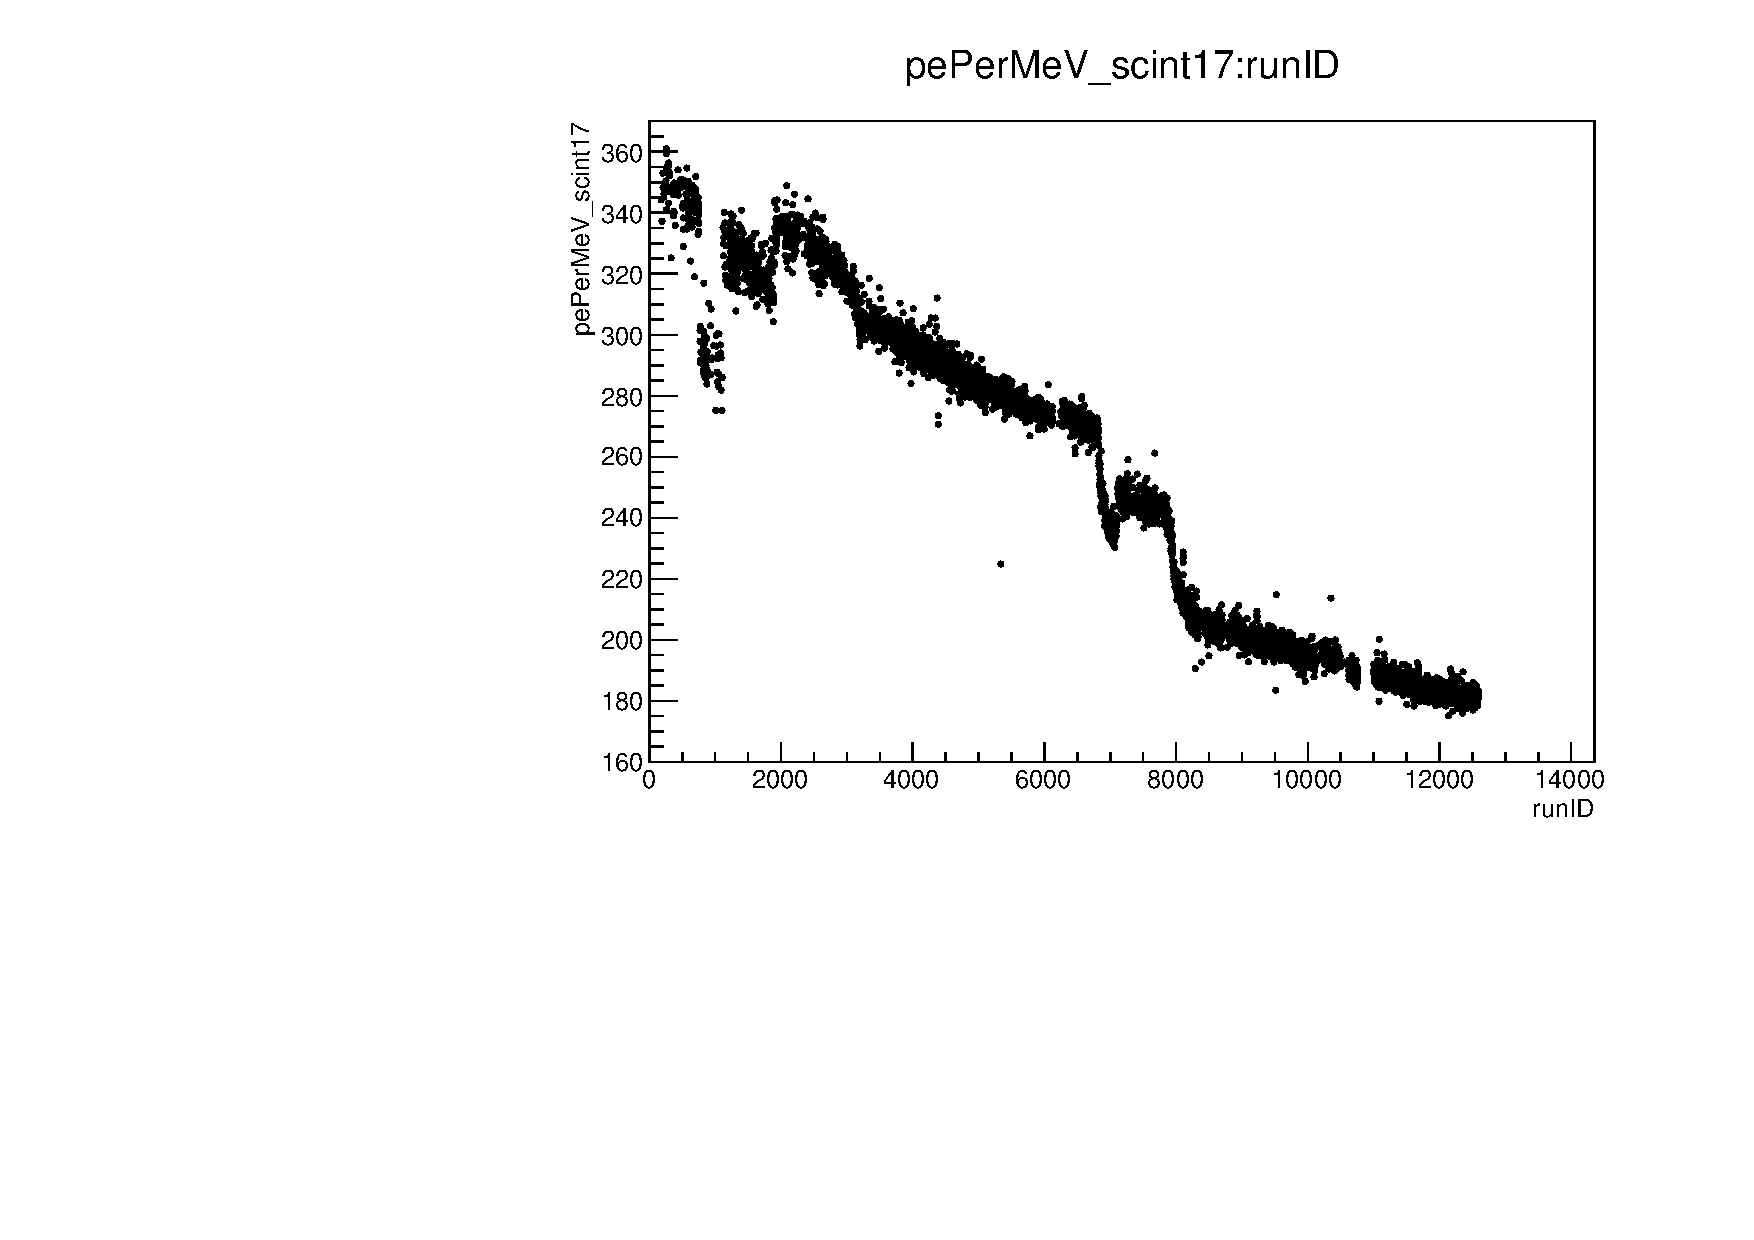
\includegraphics[width=0.45\textwidth]{scint17_allRuns.pdf} &
		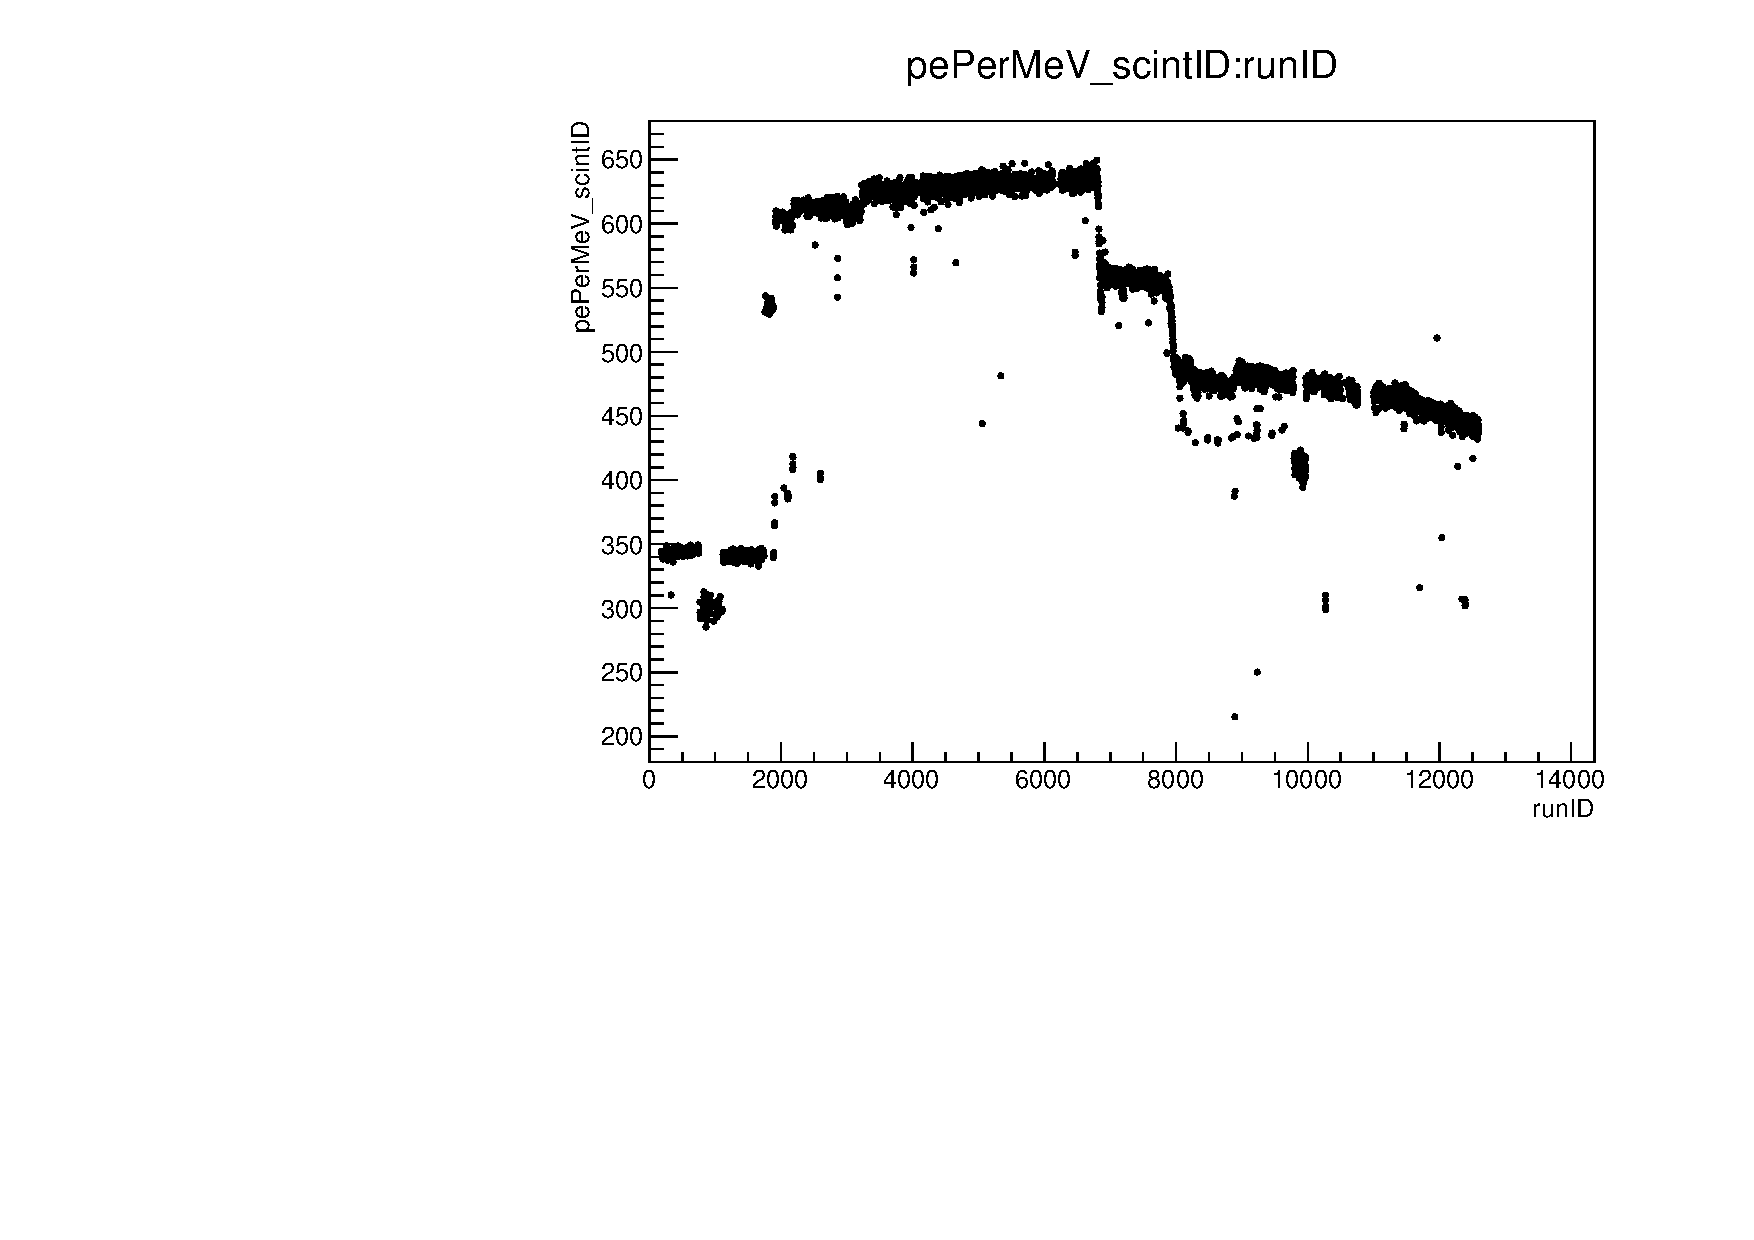
\includegraphics[width=0.45\textwidth]{scintID_allRuns.pdf} \\
		\hline
		\rotatebox[origin=c]{90}{$\text{PE}_{\text{cheren}}/\SI{}{\mega\electronvolt}$} &
		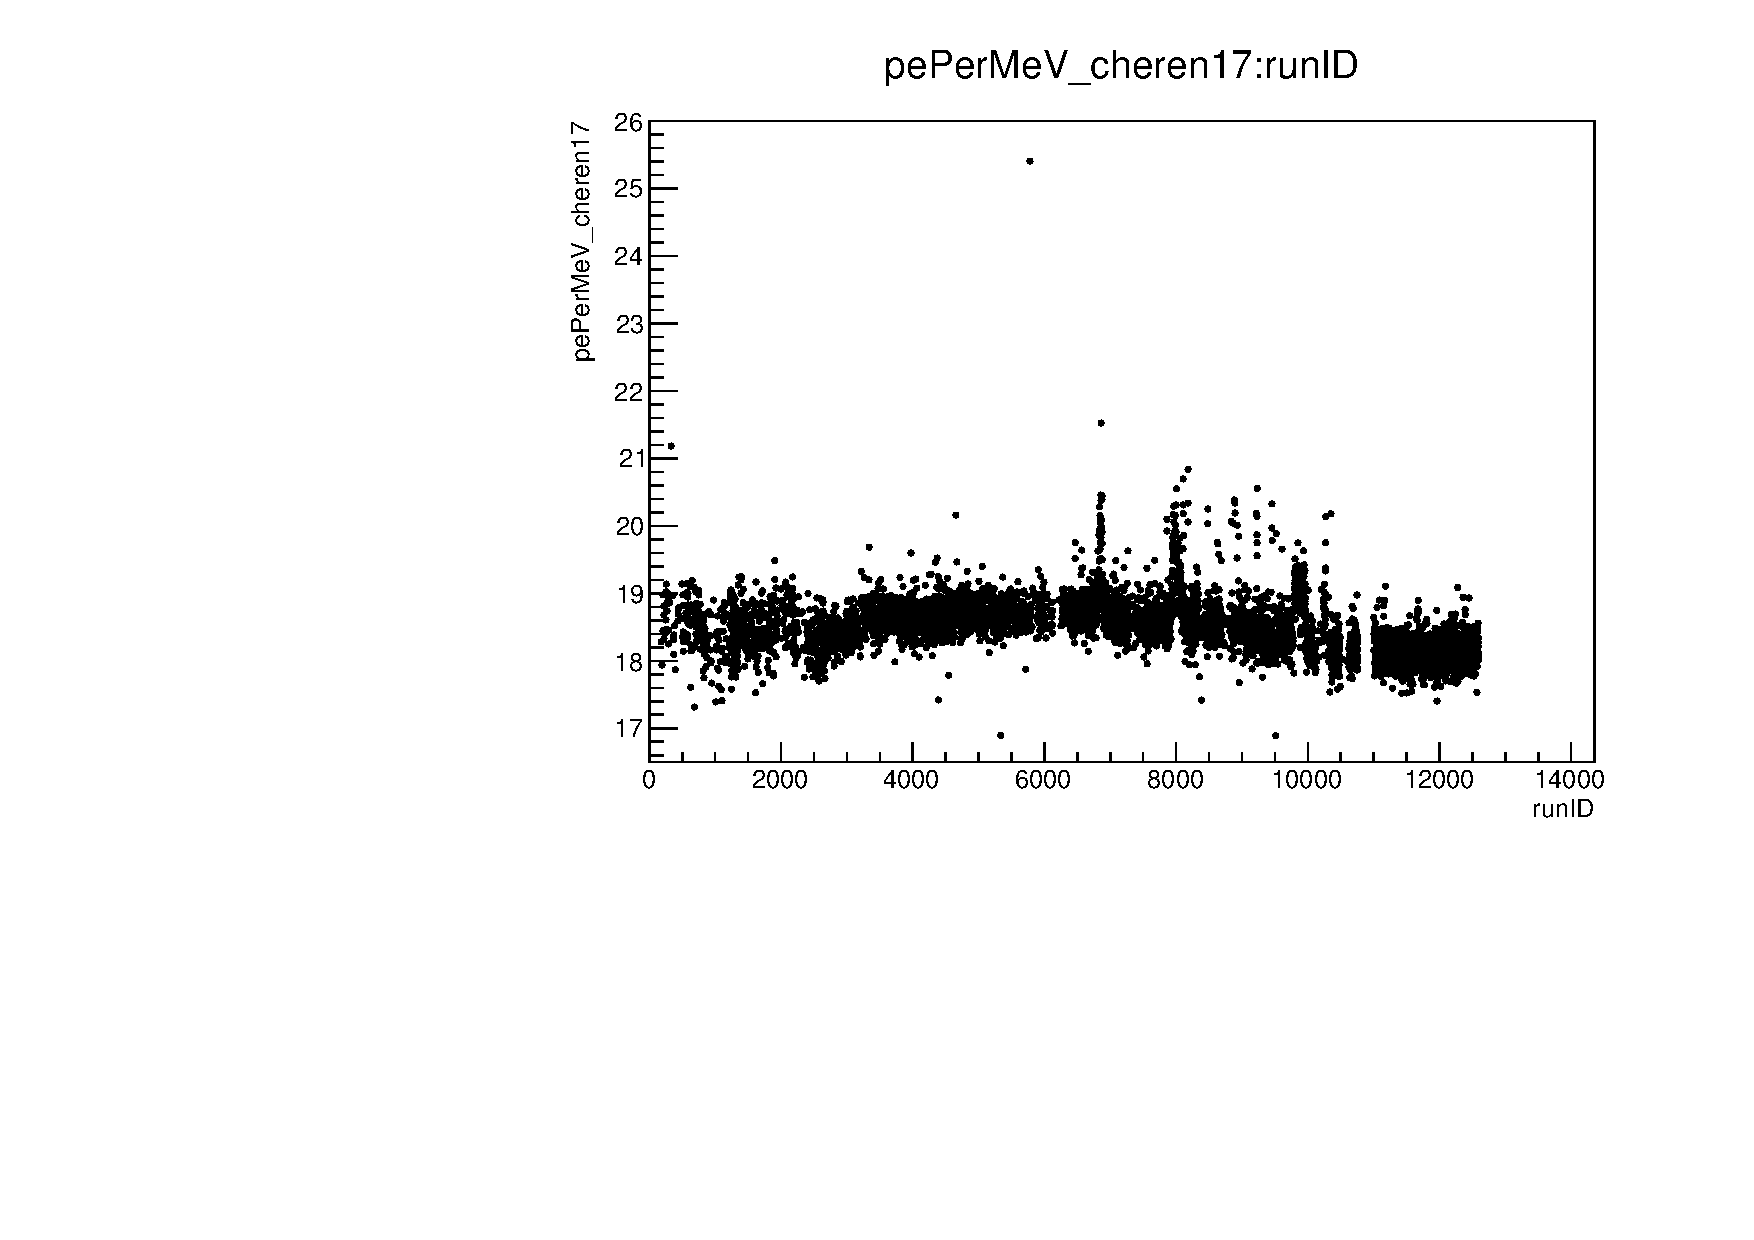
\includegraphics[width=0.45\textwidth]{cheren17_allRuns.pdf} &
		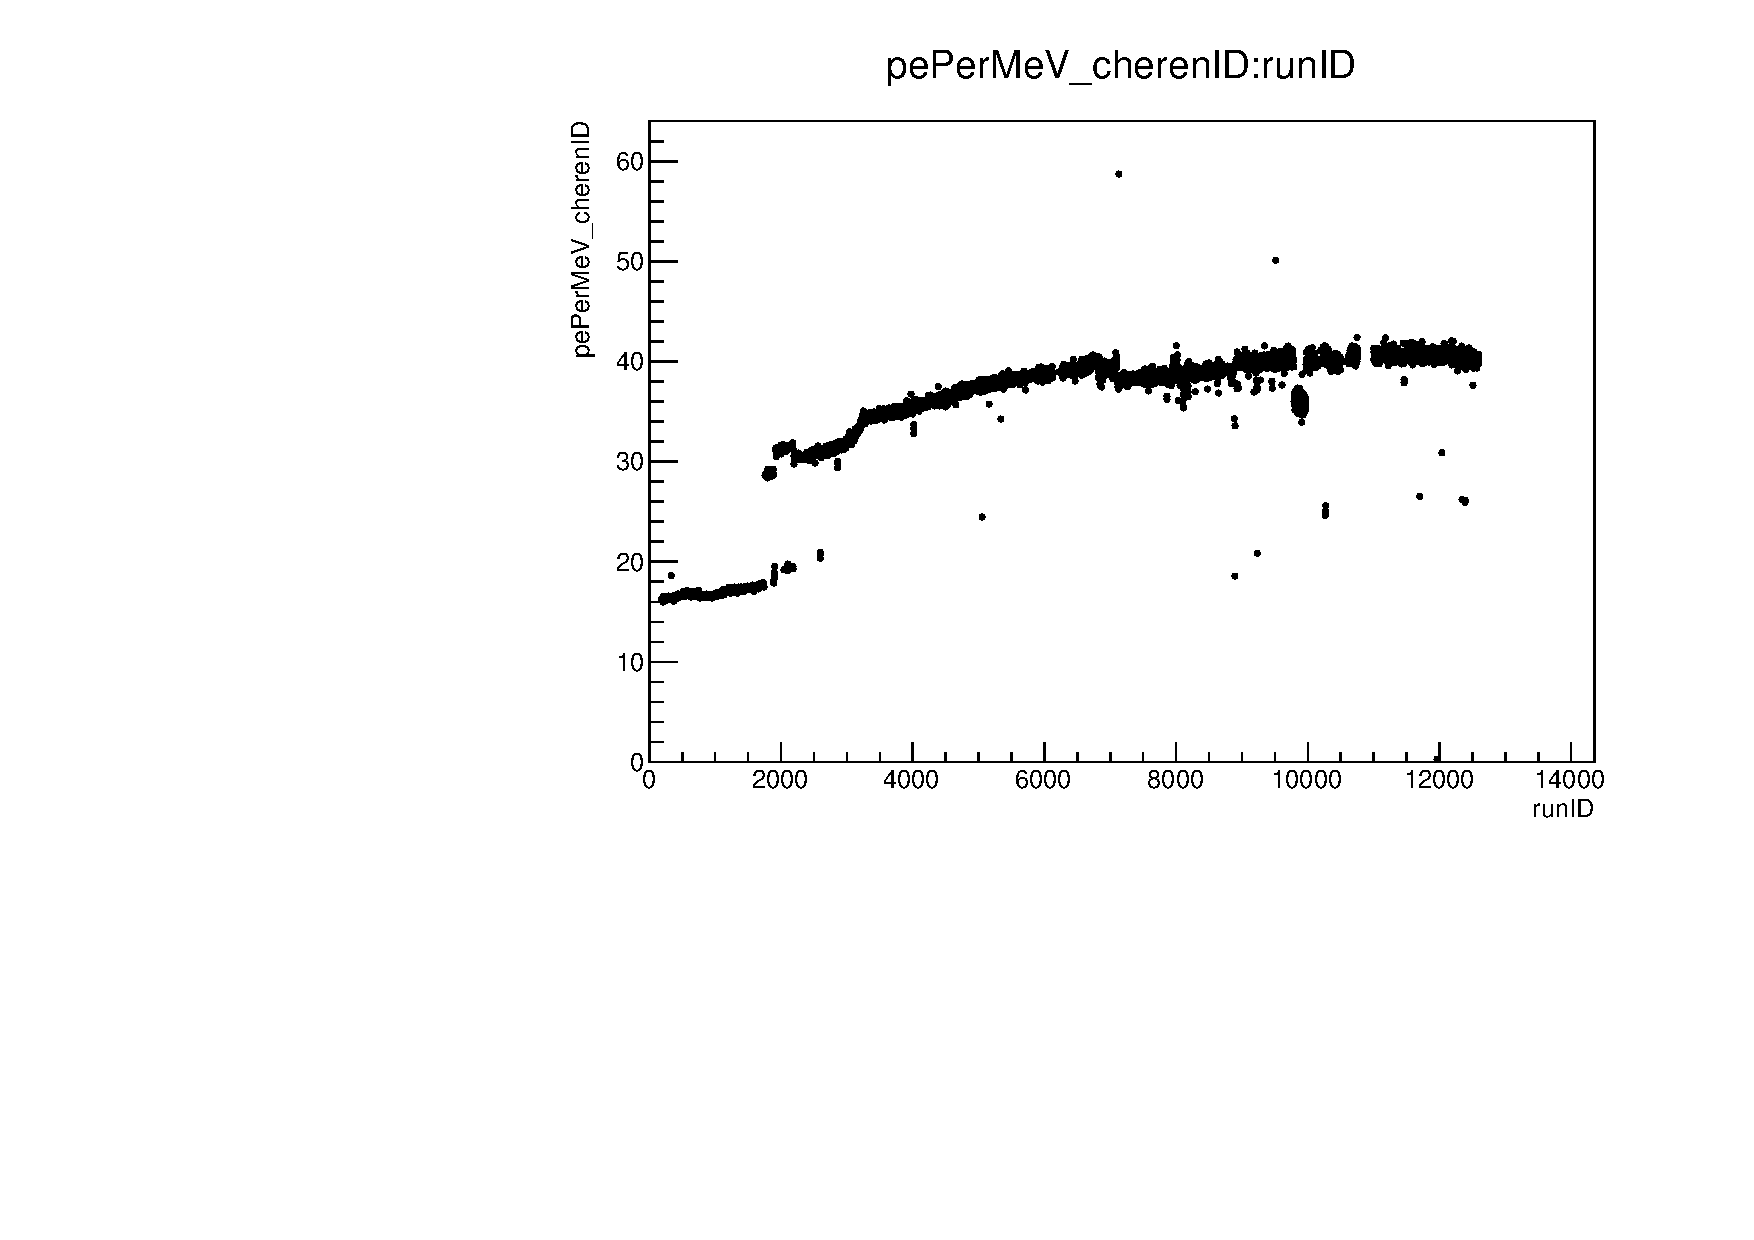
\includegraphics[width=0.45\textwidth]{cherenID_allRuns.pdf} \\
		\hline
	\end{tabular}
\end{frame}

\begin{frame}
	\frametitle{PE/MeV for all runs (KAT energy)}
	\begin{columns}[t]
		\column{0.5\textwidth}
		$\text{PE}_{\text{scint}}/\SI{}{\mega\electronvolt}$ (TotalCharge17)
		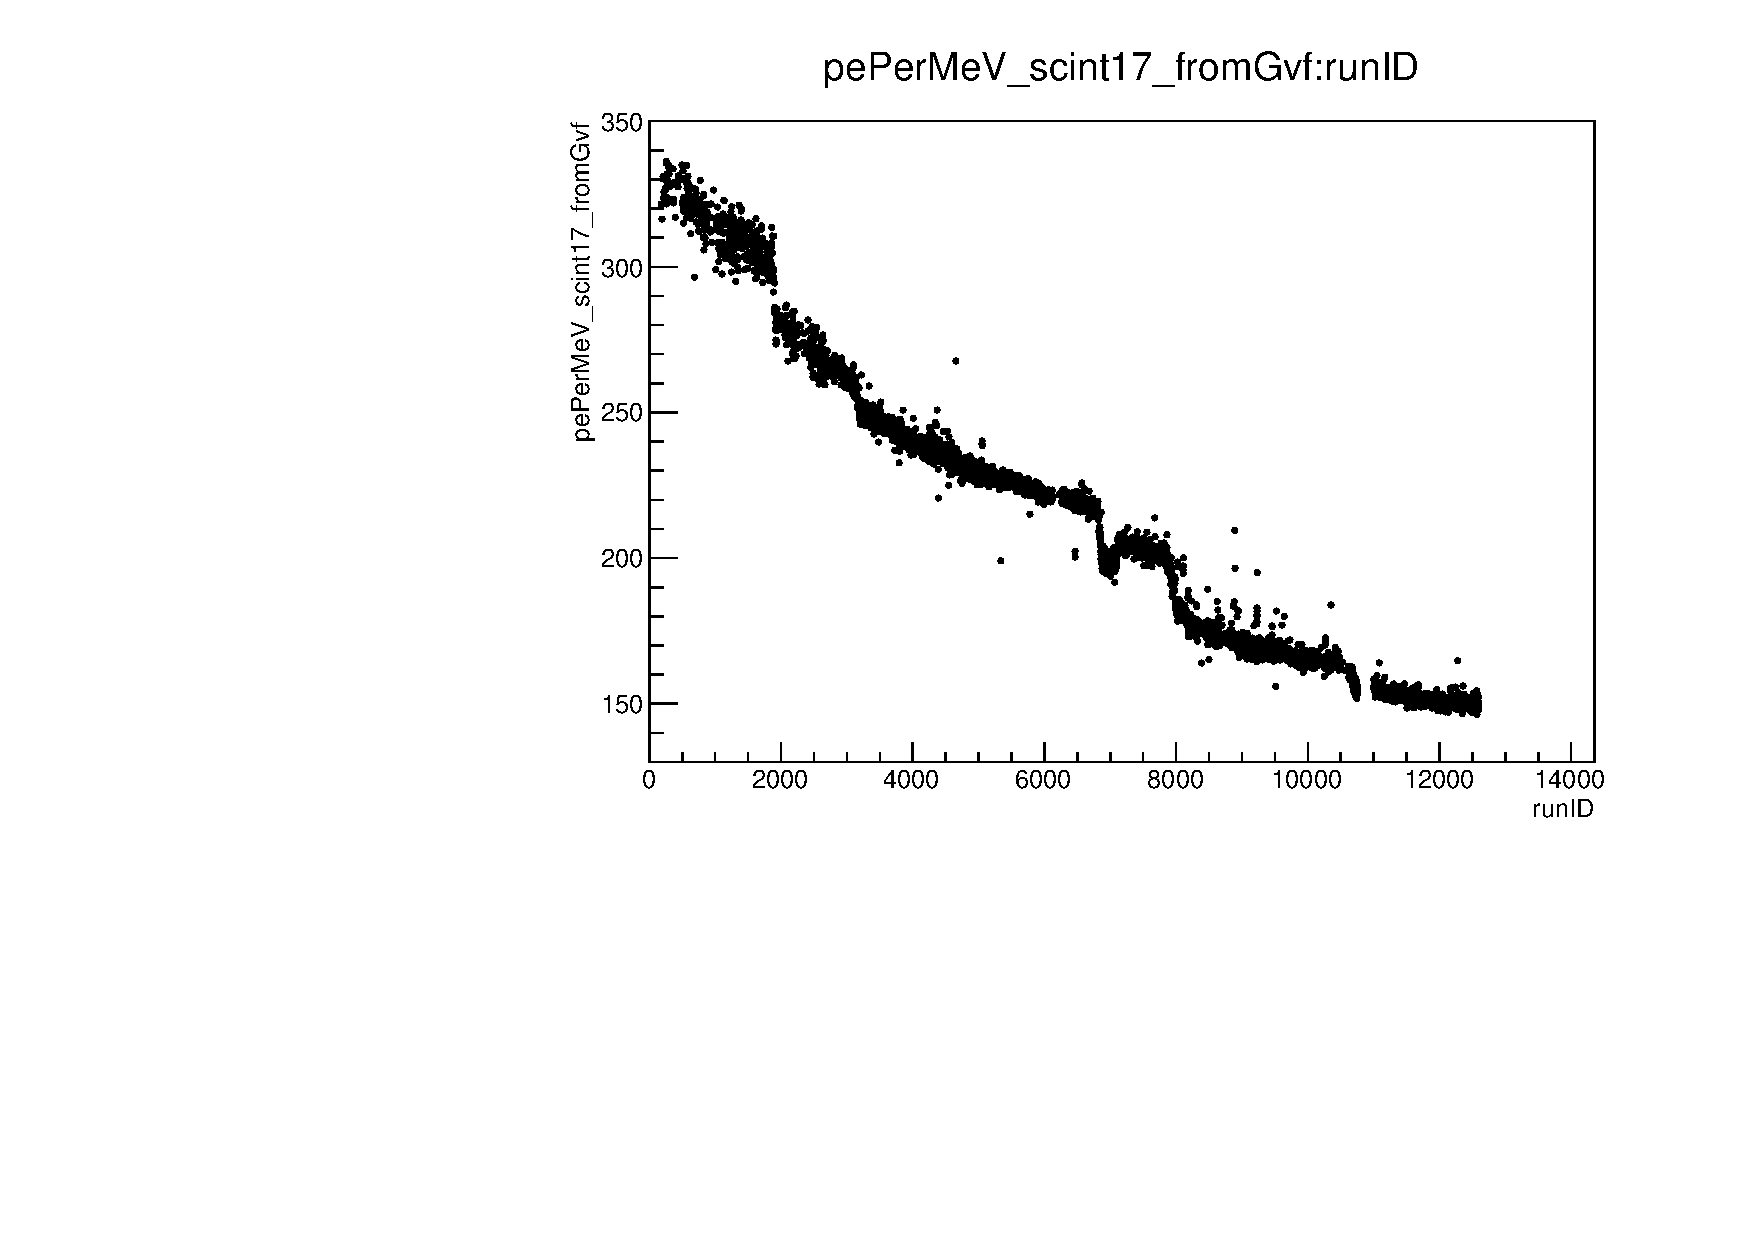
\includegraphics[width=\textwidth]{scint17_fromGvf_allRuns.pdf}
		\column{0.5\textwidth}
		$\text{PE}_{\text{scint}}/\SI{}{\mega\electronvolt}$ (TotalChargeID)
		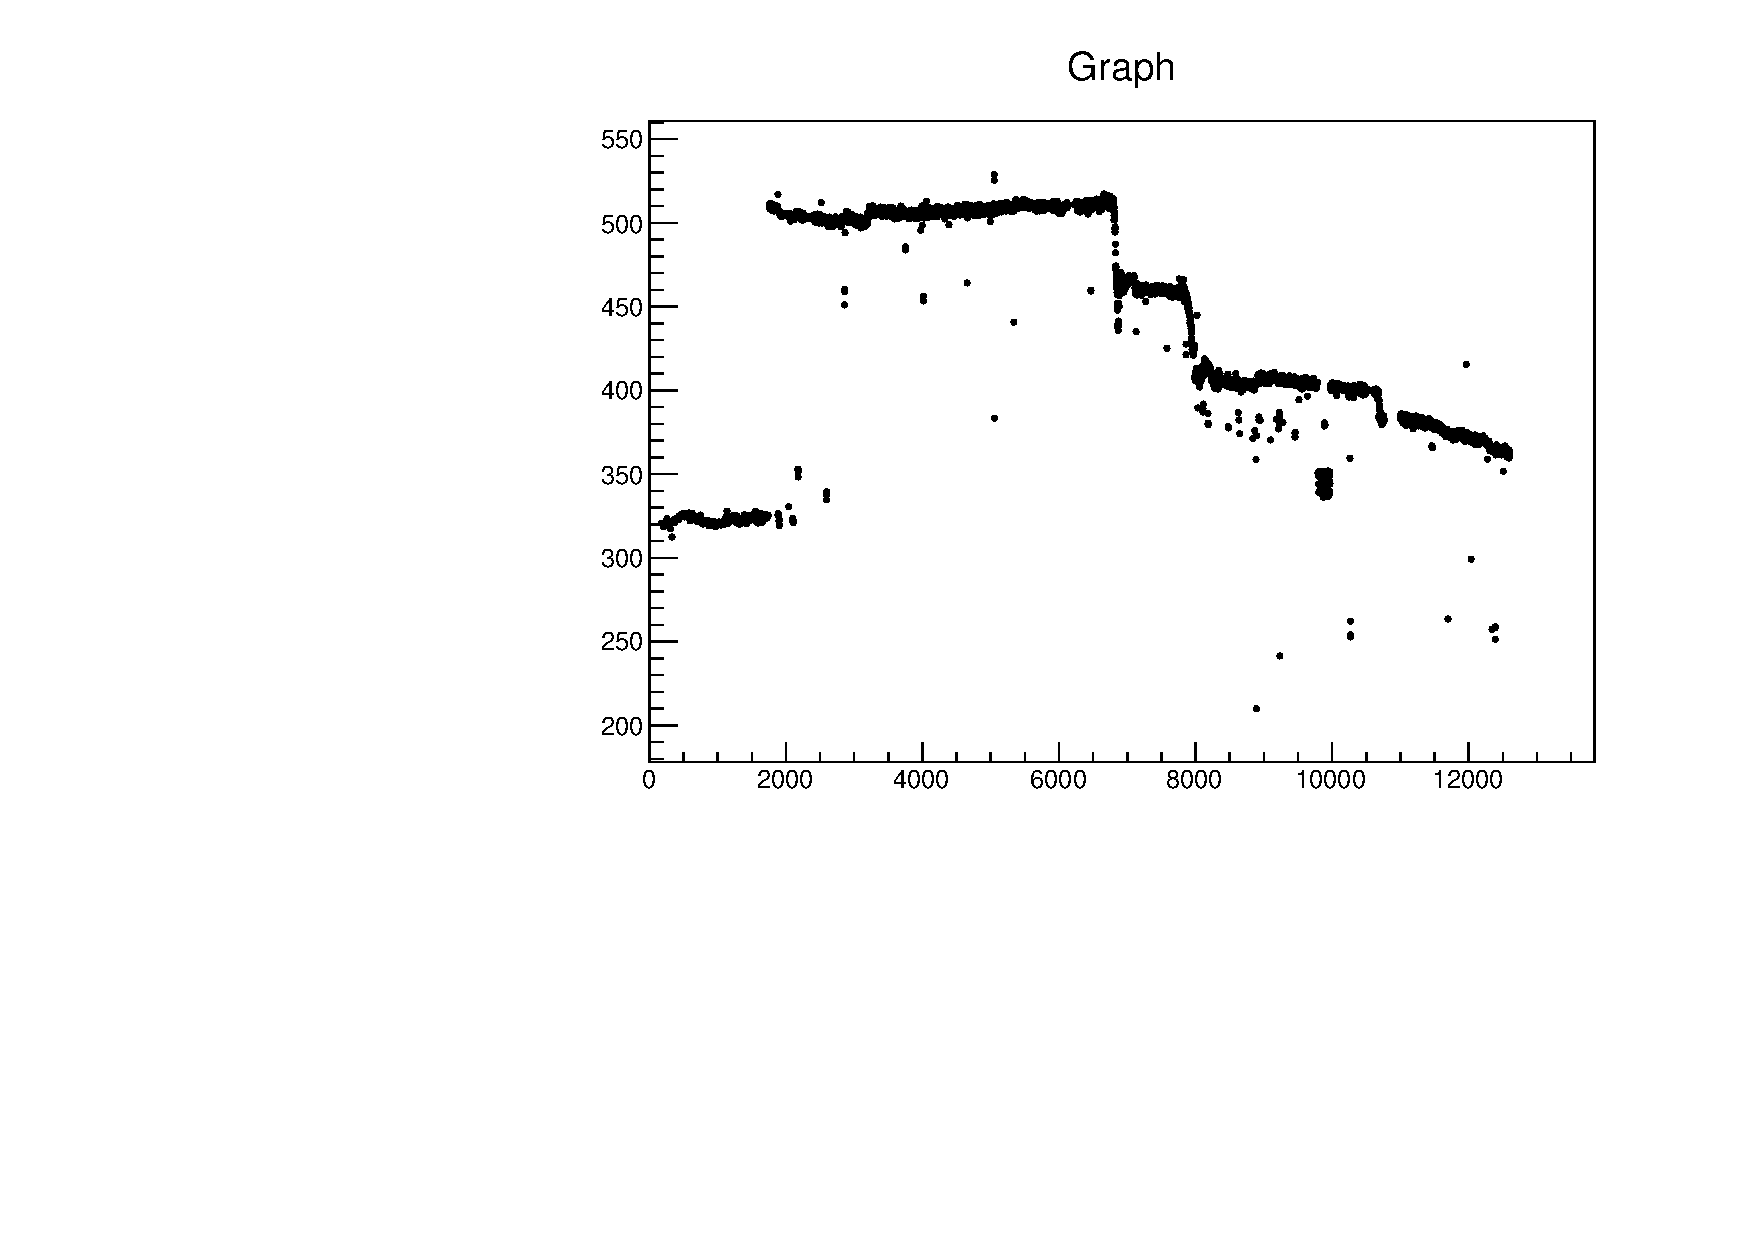
\includegraphics[width=\textwidth]{scintID_fromGvf_allRuns.pdf}
	\end{columns}
\end{frame}

\section{Neutrino Directionality}

\begin{frame}
	\frametitle{Test with muon data}
	Neutrino directionality algorithm was previously tested against KamLAND Muon
	Fitter using cosmic ray muon data
	\begin{figure}
		\centering
		\begin{subfigure}[h]{0.45\textheight}
			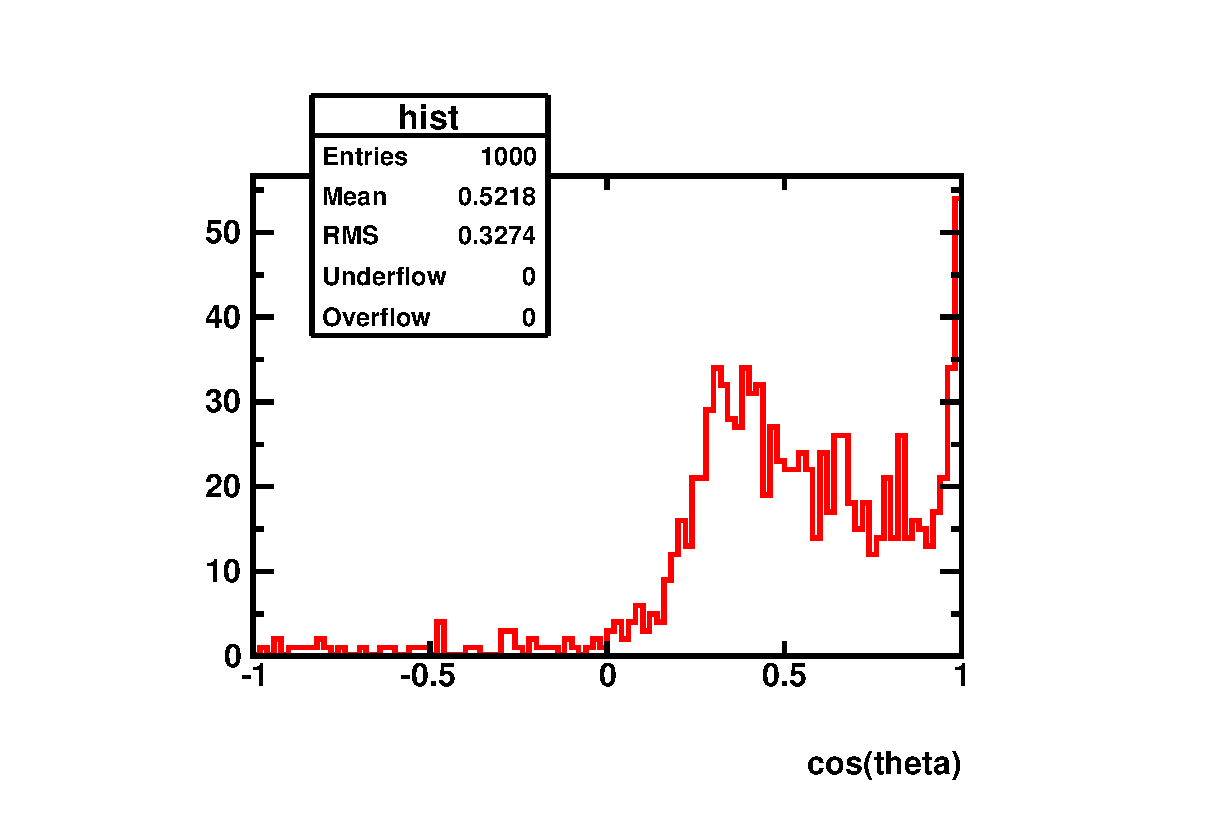
\includegraphics[width=\textwidth]
			{analyzed_rtq_atm_muon_run005000_badnessMax20_agreementWithMuonFitter}
			\caption{No cut}
		\end{subfigure}
		\begin{subfigure}[h]{0.45\textheight}
			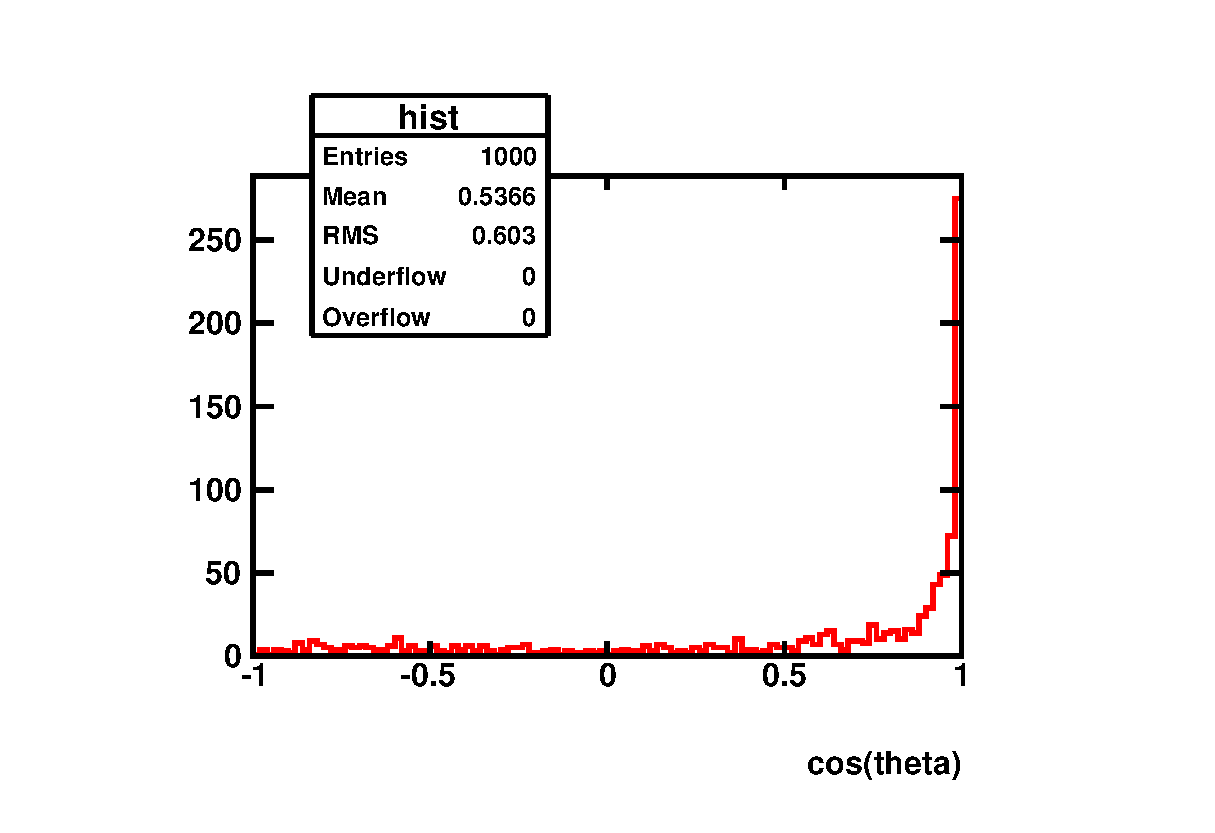
\includegraphics[width=\textwidth]
			{analyzed_rtq_atm_muon_run005000_badnessMax20_noEarlyNorLateHits_agreementWithMuonFitter}
			\caption{Prepulse cut}
		\end{subfigure}
		\caption{Agreement between Neutrino \& Muon Fitters for 1000 muons in run 5000.}
	\end{figure}
	Found prepulsing of PMTs greatly affects direction algorithm.
\end{frame}

\begin{frame}
	\frametitle{PMT Prepulsing}
	PMT prepulsing is seen at ~few \% level
	\begin{figure}
		\centering
		\begin{subfigure}[h]{0.45\textwidth}
			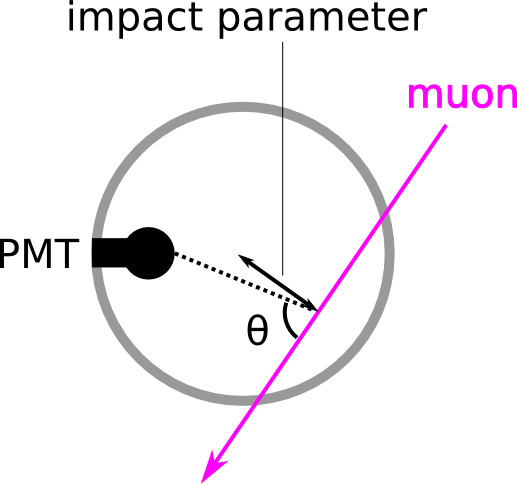
\includegraphics[width=\textwidth]{pmt_angle_wrt_muon}
		\end{subfigure}
		\begin{subfigure}[h]{0.45\textwidth}
			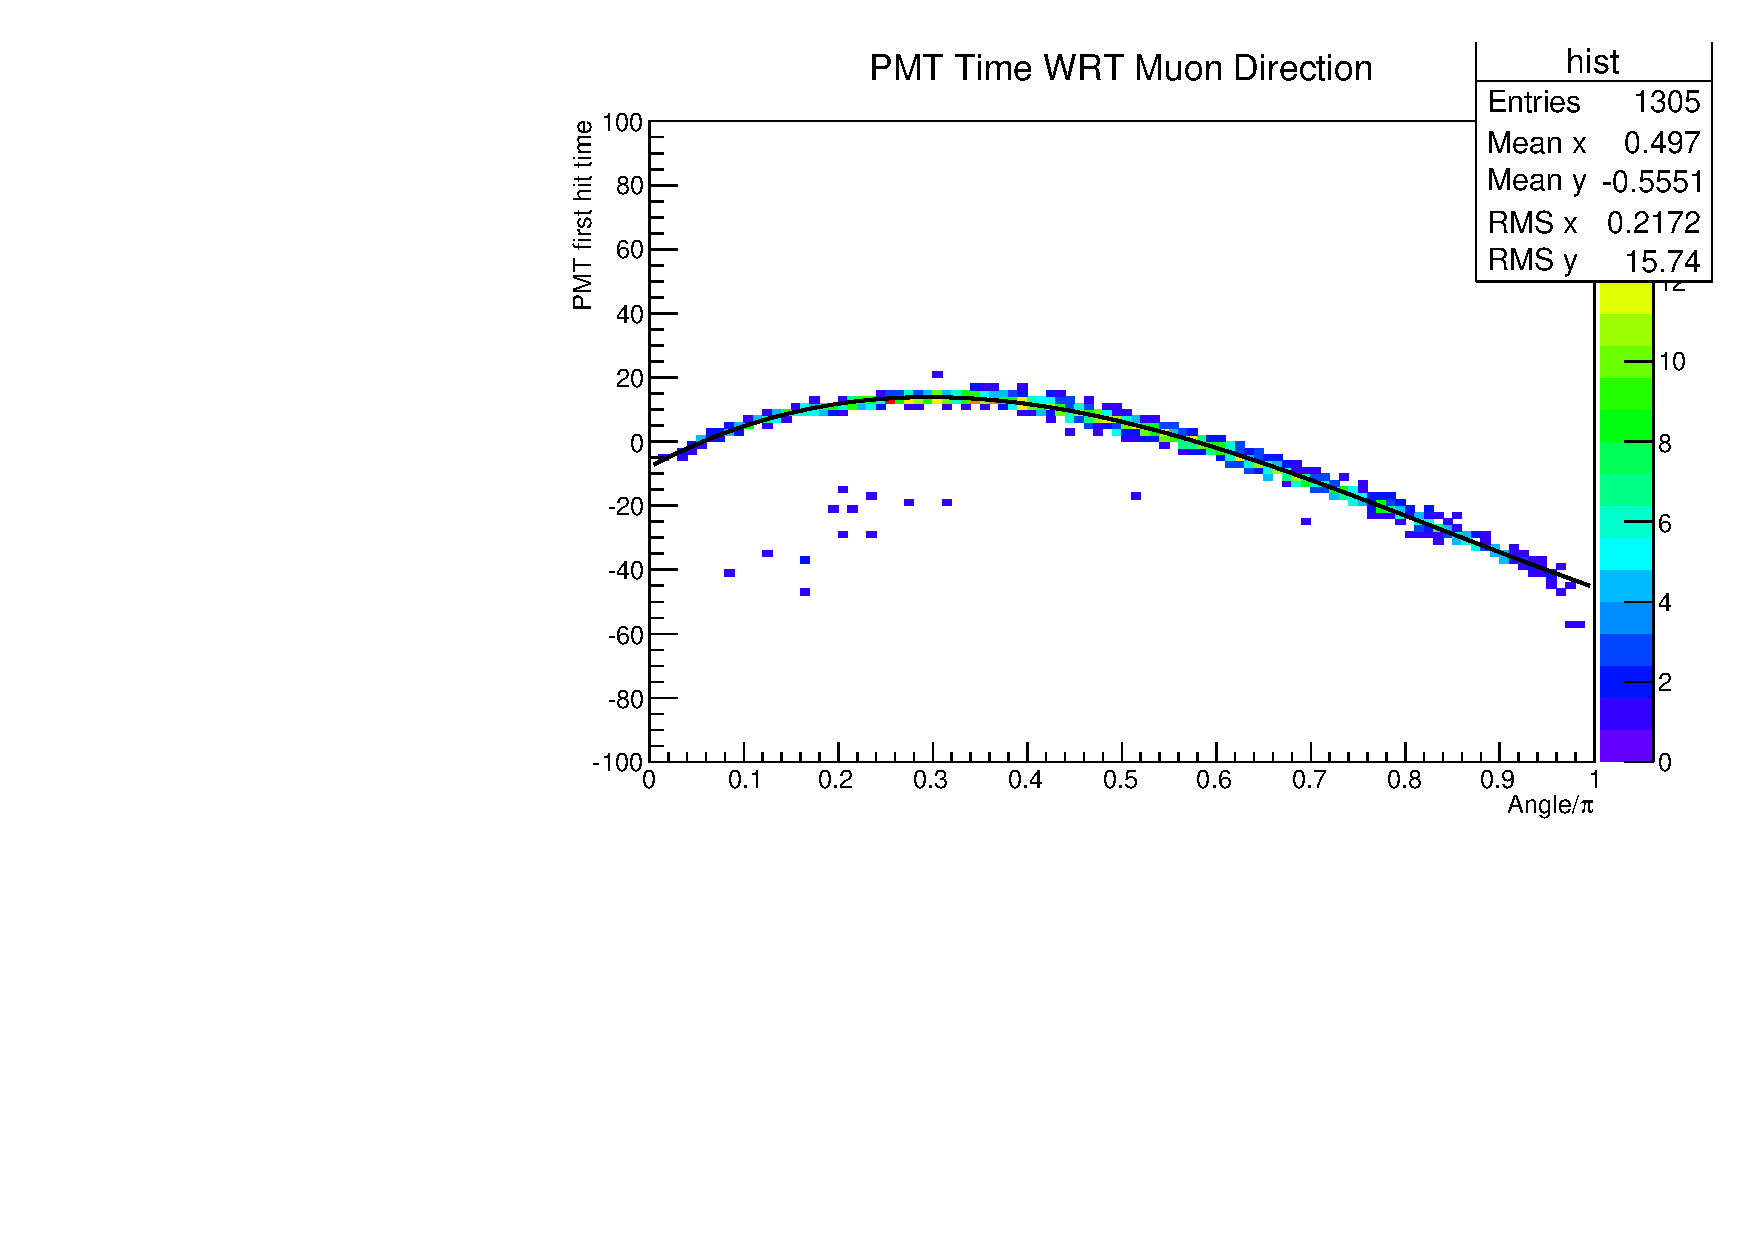
\includegraphics[width=\textwidth]{analyzed_rtq_run005000_hitTimePositions_0prepulseCutPassAt3SigOfNeighbors.pdf}
			\caption{Single muon event with clear prepulse observed}
		\end{subfigure}
	\end{figure}
\end{frame}

\begin{frame}
	\frametitle{How to resolve prepulsing?}
	\begin{itemize}
		\item Throw away PMT hits that look early compared to surrounding
			neighbor PMTs. \\
			$\rightarrow$ Throwing away information! \\
			$\rightarrow$ Cannot remove clusters of prepulsing PMTs
		\item Can we do better? \\
			$\rightarrow$ Maybe just throw away first small pulse in multi-pulse
			waveform and use first big pulse as PMT hit time?
	\end{itemize}
\end{frame}

\begin{frame}
	\frametitle{Algorithm to filter prepulse:}
	\begin{figure}
		\centering
		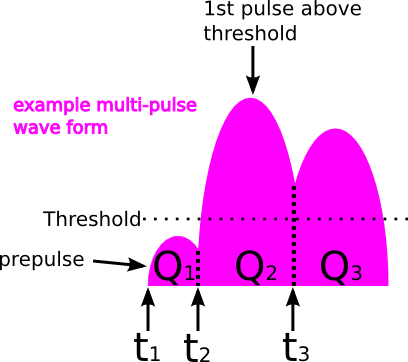
\includegraphics[height=0.45\textheight]{prepulse}
	\end{figure}
	Algorithm:
	\begin{enumerate}
		\item threshold $\equiv 0.05 \times$ (charge of largest pulse $Q_2$)
		\item choose first pulse above threshold
		\item let hit time = $t_2$
		\item let charge = $Q_1 + Q_2 + Q_3$
	\end{enumerate}
\end{frame}

\begin{frame}
	\frametitle{Unfortunately, naively cutting first "small" and using next "large" pulse does not work!}
	\framesubtitle{204 events, runs \numrange[range-phrase=--]{5000}{5009}}
	\begin{columns}[t]
		\column{0.5\textwidth}
		Using first hits
		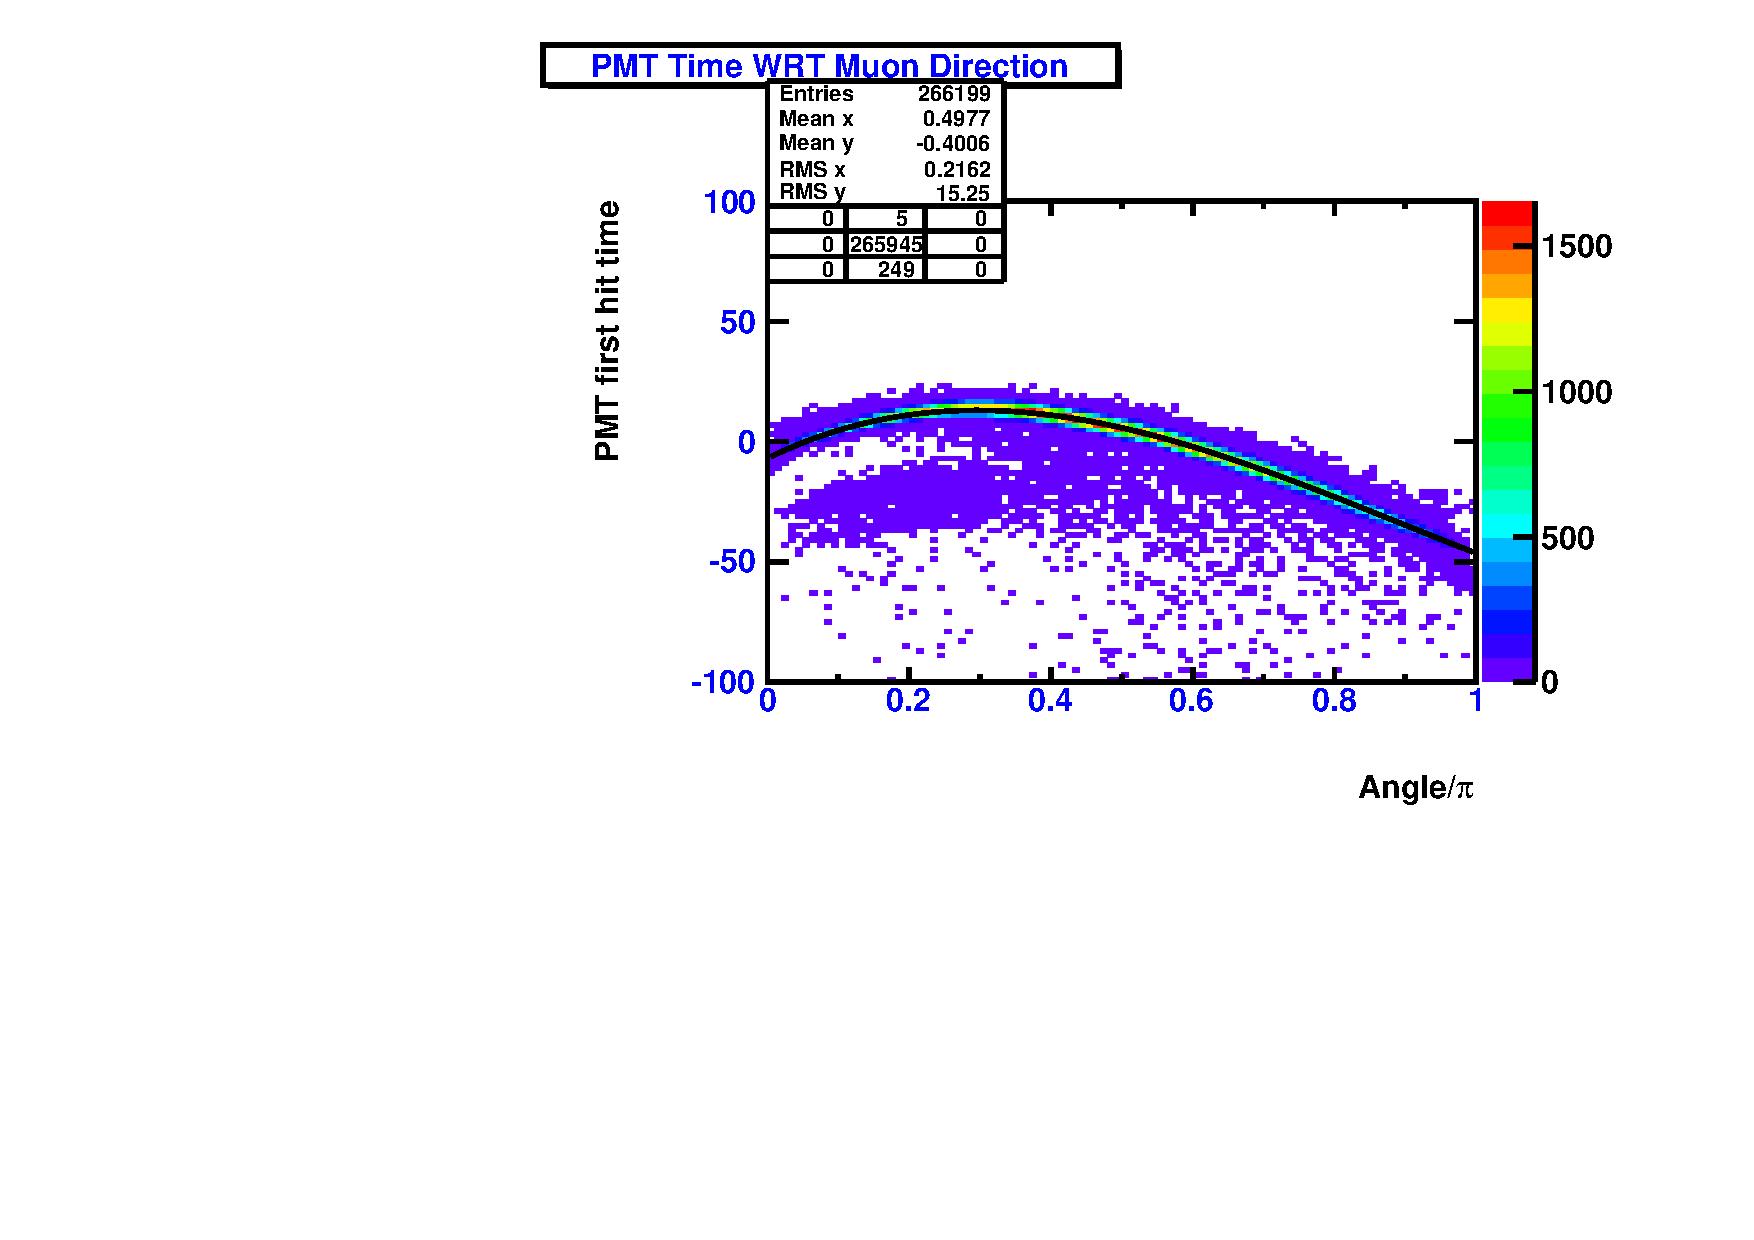
\includegraphics[width=1.0\textwidth]{analyzed_rtq_atm_mu_run005000_test_hitTimePositions_includeEarlyLateHits.pdf}
		\column{0.5\textwidth}
		Using first large pulse hits
		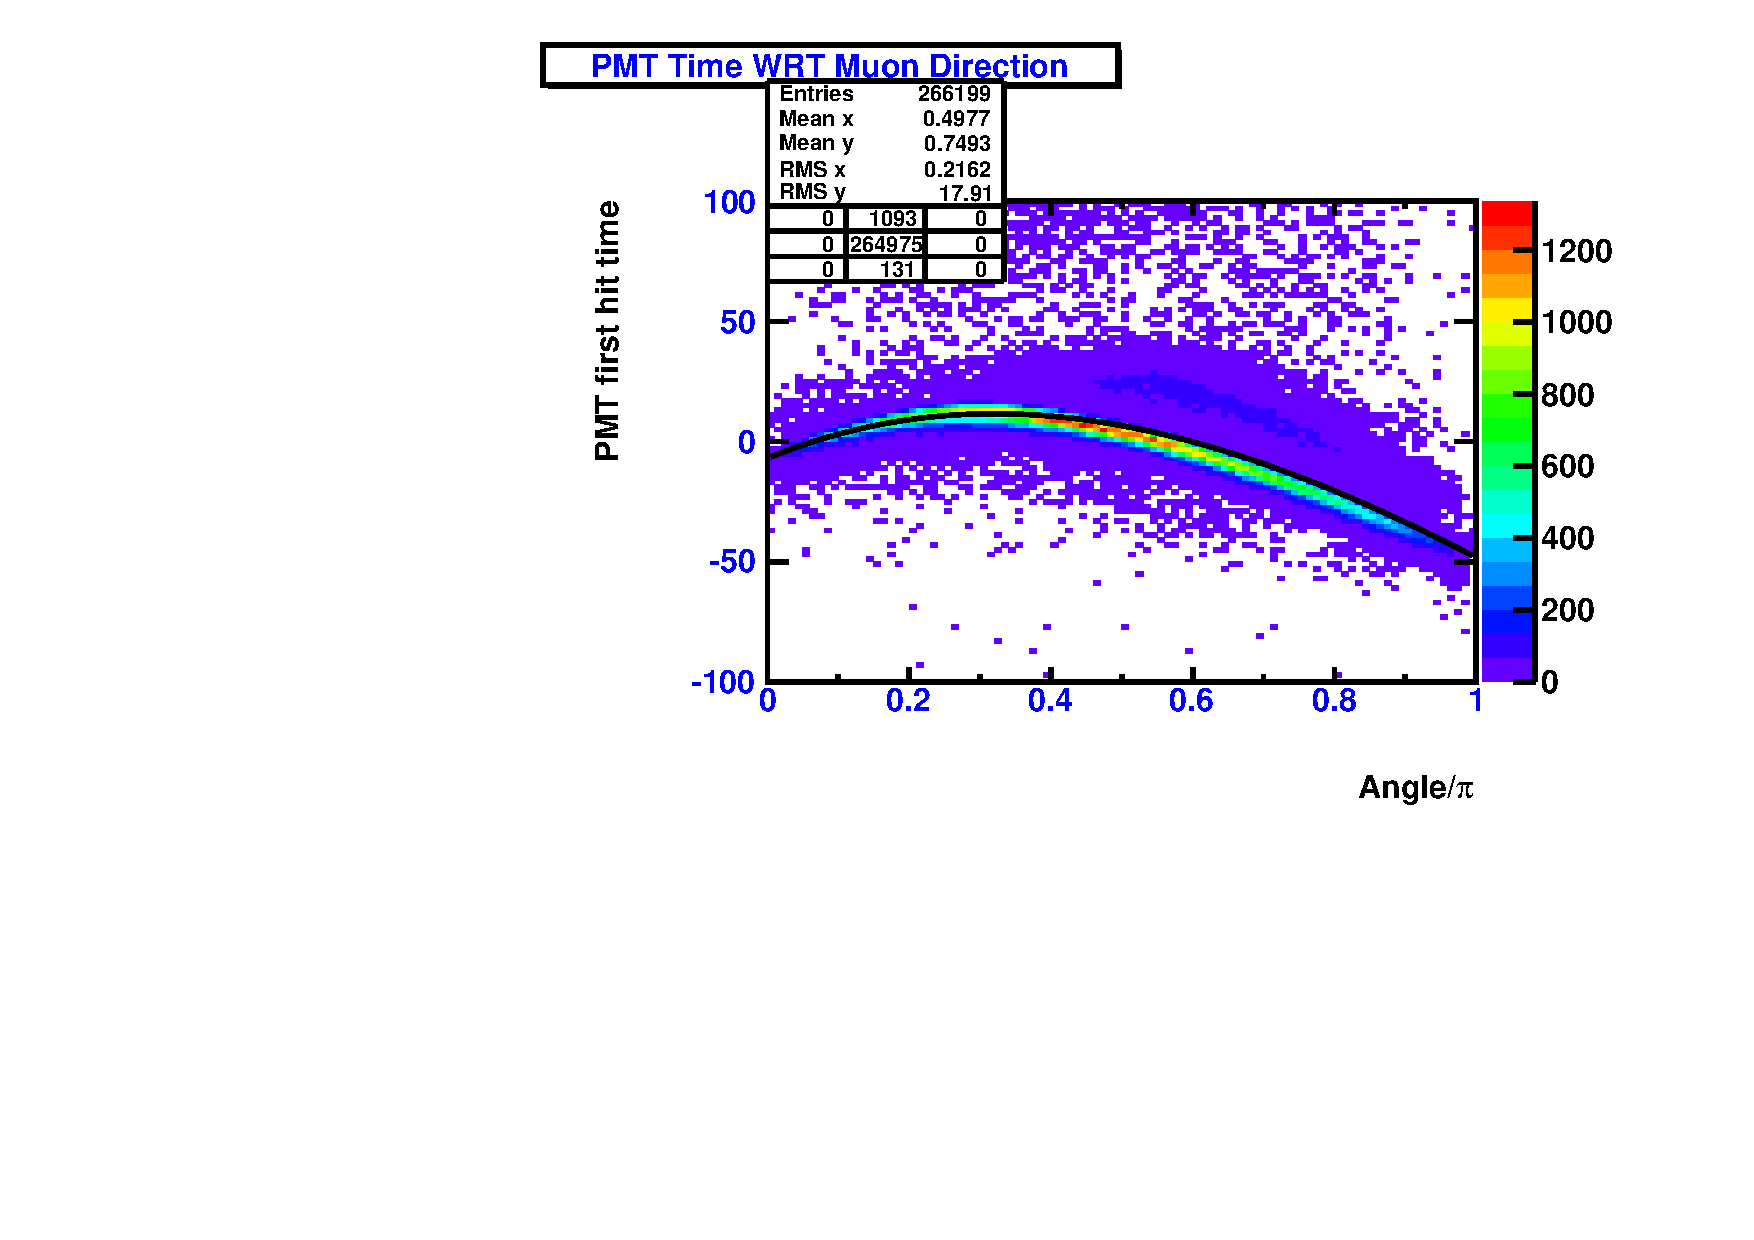
\includegraphics[width=1.0\textwidth]{analyzed_rtq_atm_mu_run005000_multiPulse_test_hitTimePositions_includeEarlyLateHits.pdf}
	\end{columns}
\end{frame}

\begin{frame}
	\frametitle{Gain Dependency of Prepulse}
	\begin{itemize}
		\item Difficult to cut all of prepulse
			\begin{itemize}
				\item Prepulse is easy to filter when pulse is from large gain
				\item But harder to filter when pulse is from mid/low gain
					(prepulse is only sometimes seen depending on pulse charge)
			\end{itemize}
	\end{itemize}
\end{frame}

\begin{frame}
	\frametitle{Improved $\nu$ fitter}
	Sensitivity to outlier hit times was reduced \\
	$\rightarrow$ $\nu$ fitter agreement with KamLAND $\mu$ fitter was improved
	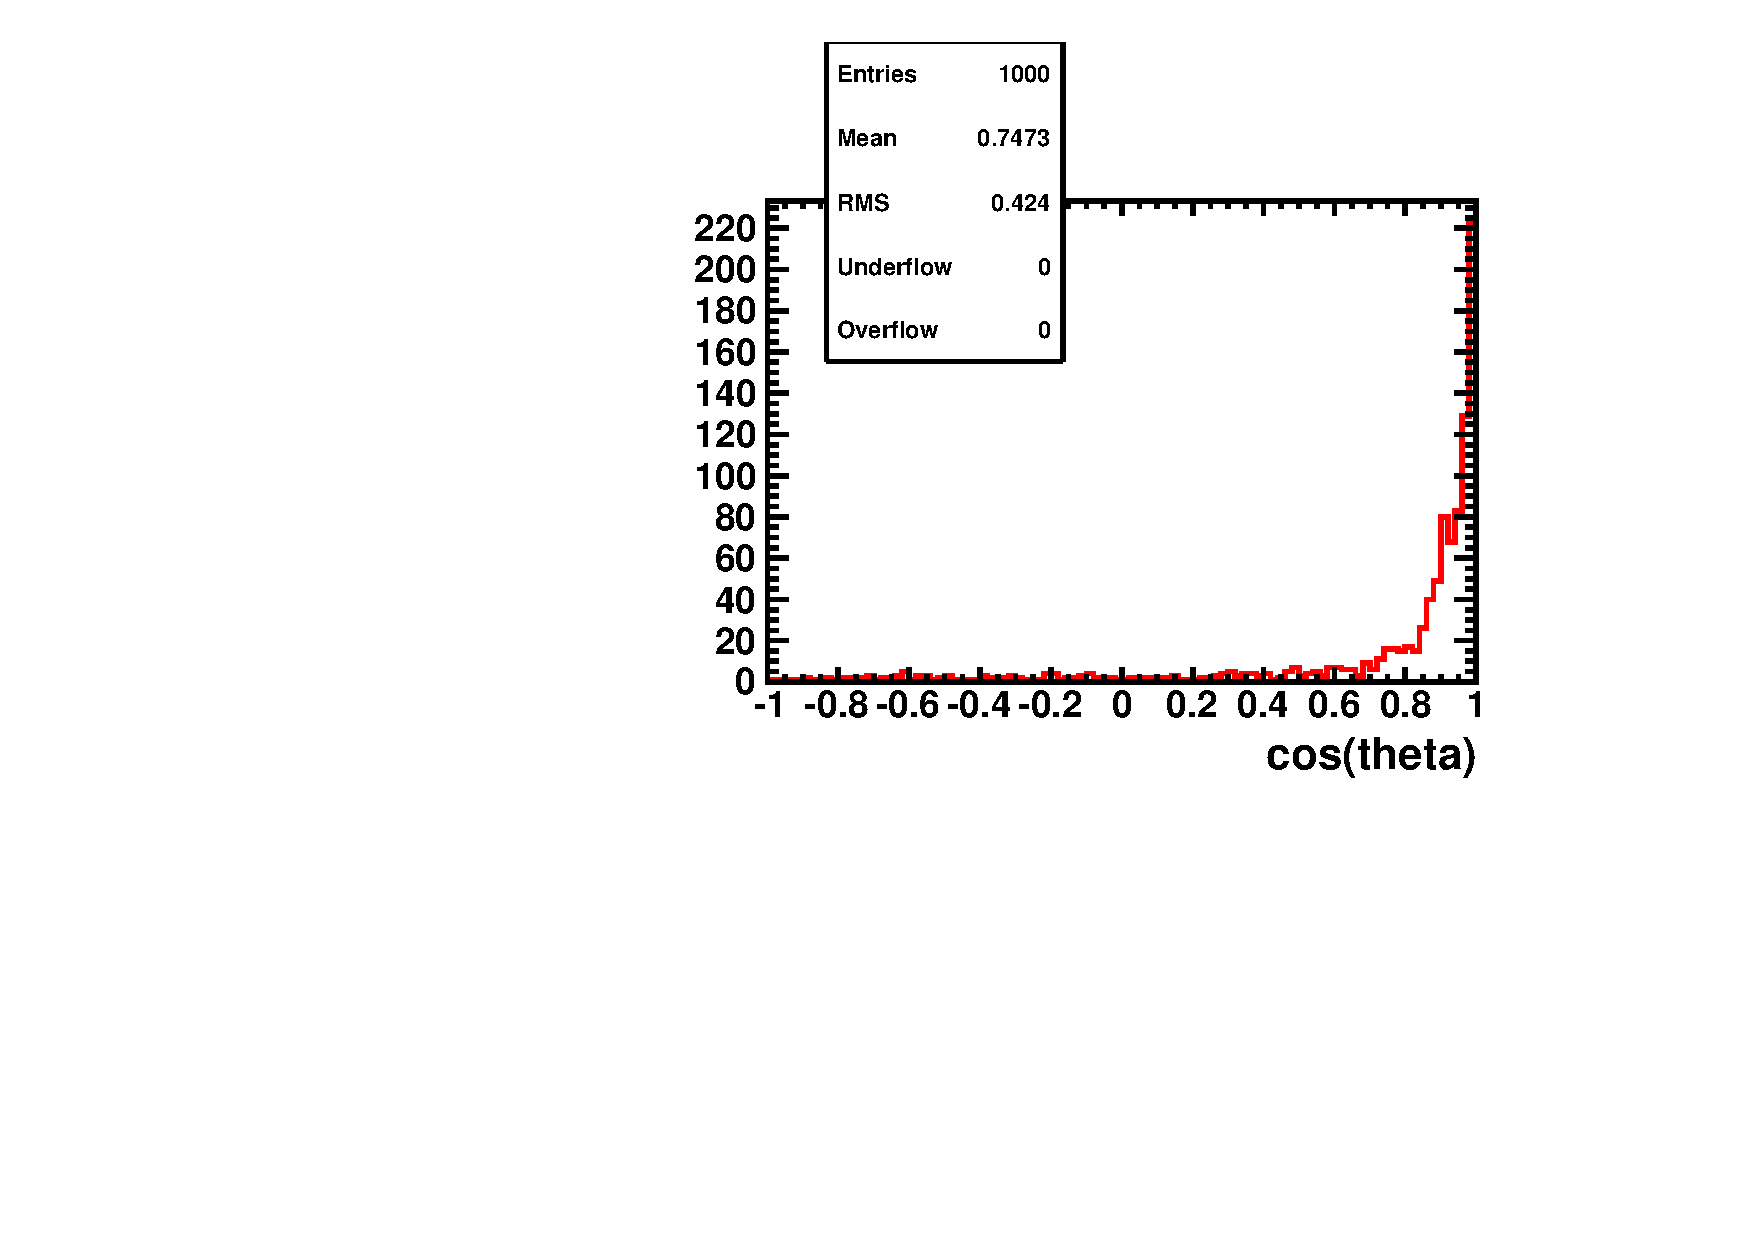
\includegraphics[width=\textwidth]{analyzed_rtq_run005000_agreementWithMuonFitter_t0Peak_prepulseCut1_0_05maxQThres_1000evts.pdf}
\end{frame}

\begin{frame}
	\frametitle{Test neutrino direction algorithm for simulated events (no prepulsing)}
	Procedure:
	\begin{enumerate}
		\item Use GENIE to let $\nu_{e}$
			(\SIrange[range-phrase=--]{0.1}{5}{\giga\electronvolt}) interact
			with main LS nuclei ($^{1}$H, $^{12}$C) 
		\item Use KLG4 to simulate detector response using uniform distribution
			of events in ID (no residual nucleus / no prepulsing)
		\item Place OD hit $< 5$
		\item Reconstruct event properties using neutrino fitter and
			KAT
	\end{enumerate}
\end{frame}

\begin{frame}
	\frametitle{Agreement between true/reconstructed $\nu$ angle}
	\framesubtitle{no fiducial volume cut}
	\begin{columns}[T]
		\column{0.5\textwidth}
		\ce{\nu_{e} + ^{1}H -> e^{-} + ?}
		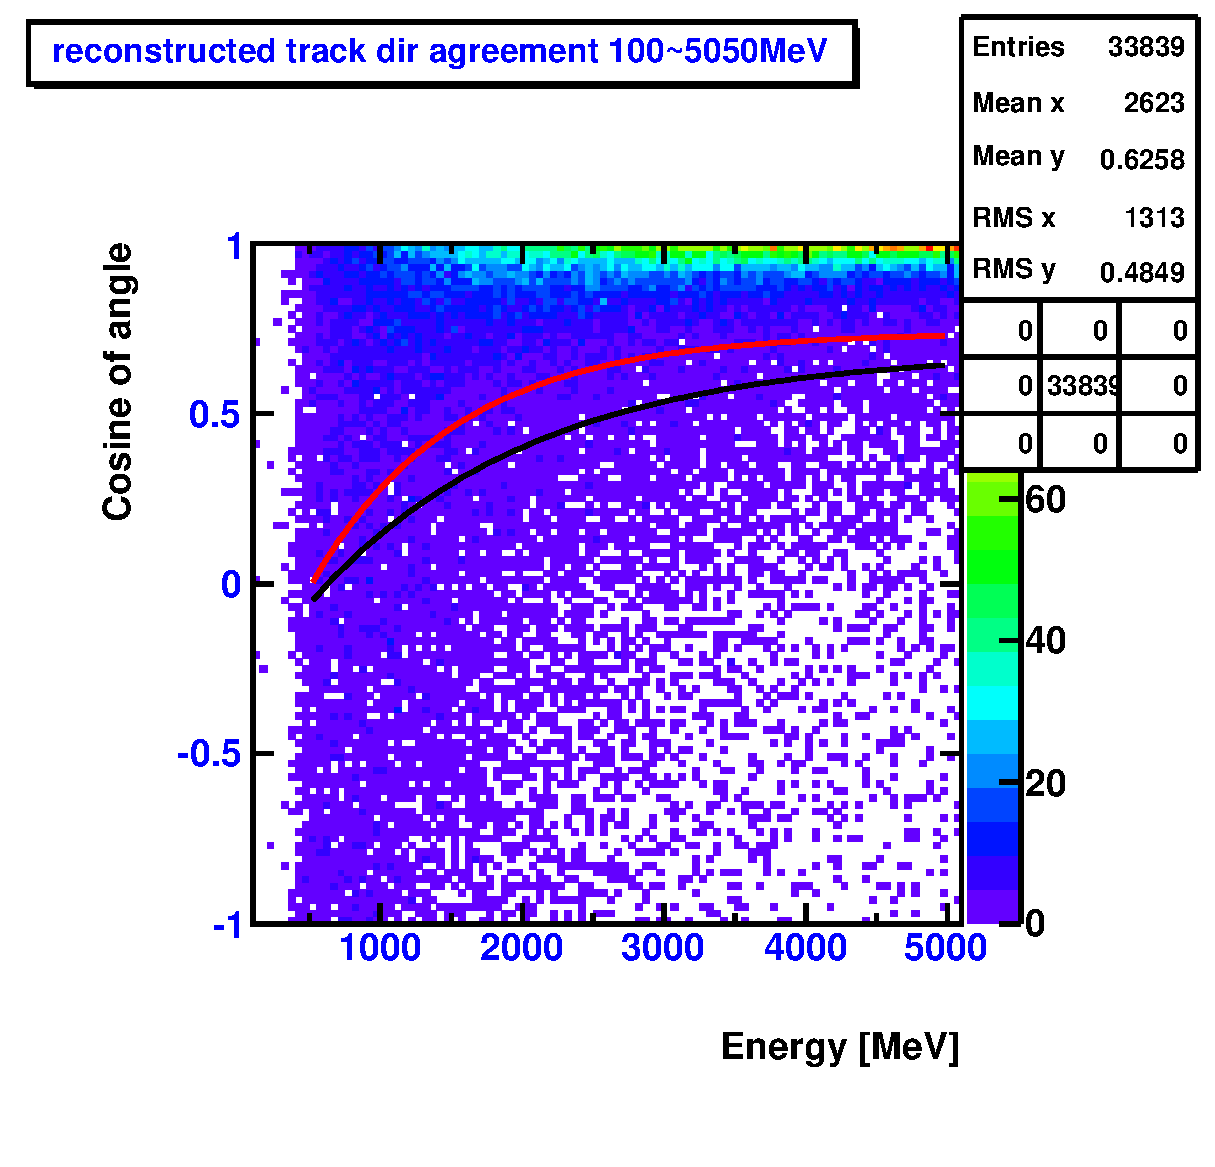
\includegraphics[width=1.0\textwidth]{analyzed_mtq_flatSpectrum_nue_H1_outerBufferFillAll_reconDirAgreementWithMtqTruthVectorVSEnergy_onlyCC.eps}
		\column{0.5\textwidth}
		\ce{\nu_{e} + ^{12}C -> e^{-} + ?}
		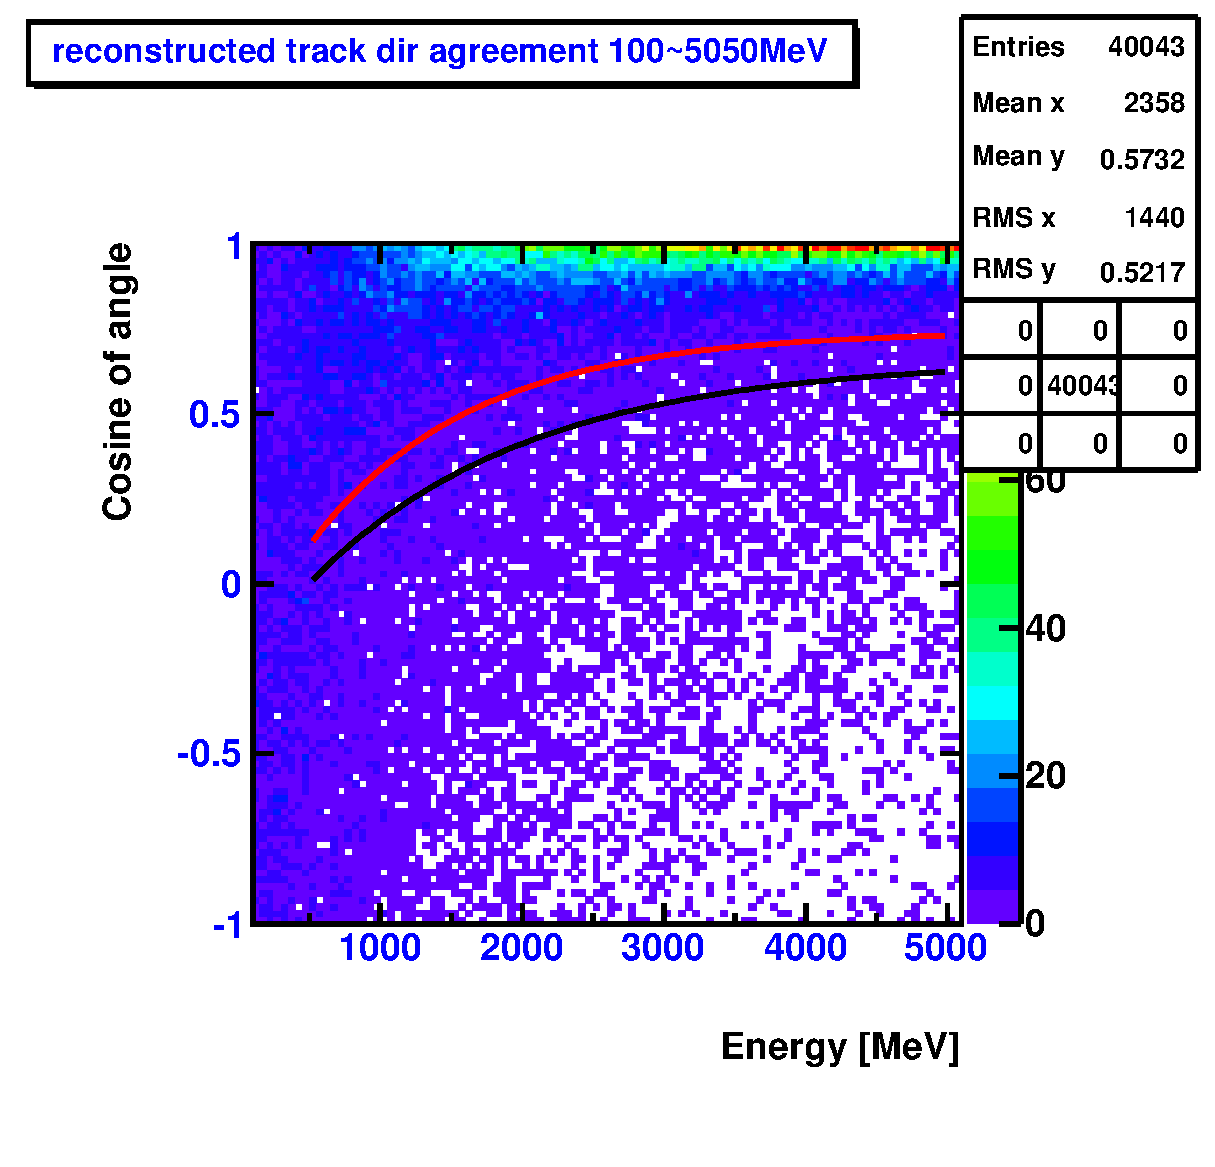
\includegraphics[width=1.0\textwidth]{analyzed_mtq_flatSpectrum_nue_C12_outerBufferFillAll_reconDirAgreementWithMtqTruthVectorVSEnergy_onlyCC.eps}
	\end{columns}
	Black line: 1$\sigma$ of reconstructed angle from $\nu$ direction \\
	Red line: 1$\sigma$ of lepton angle from $\nu$ direction
\end{frame}

\begin{frame}
	\frametitle{Agreement between true/reconstructed $\nu$ angle}
	\framesubtitle{vertex $R < \SI{600}{cm}$}
	\begin{columns}[t]
		\column{0.5\textwidth}
		\ce{\nu_{e} + ^{1}H -> e^{-} + ?}
		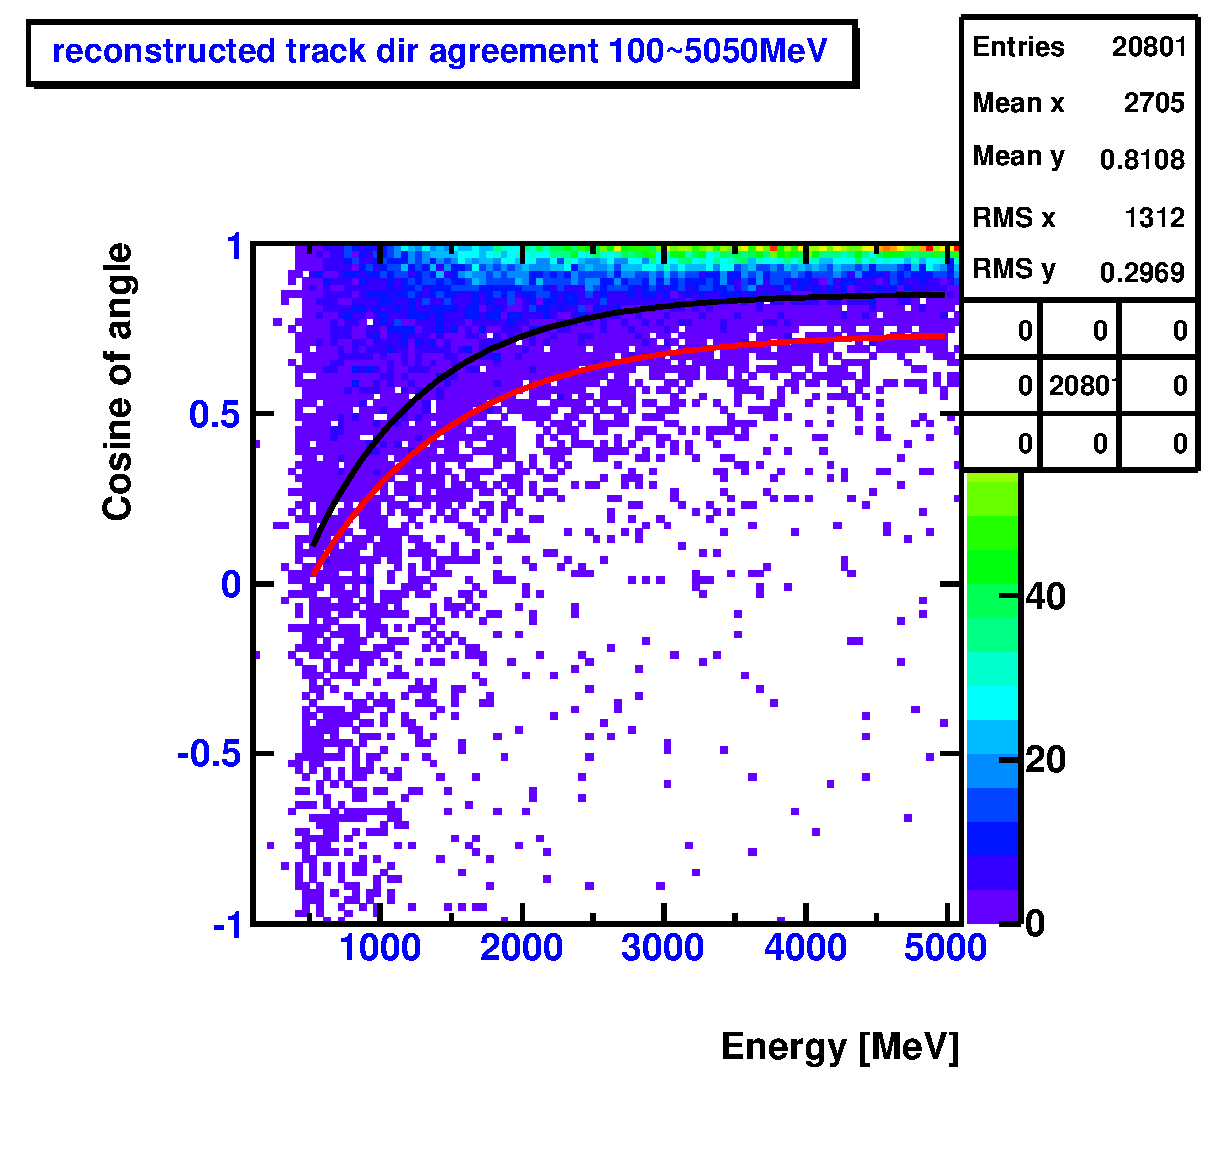
\includegraphics[width=1.0\textwidth]{analyzed_mtq_flatSpectrum_nue_H1_outerBufferFillAll_reconDirAgreementWithMtqTruthVectorVSEnergy_onlyCC_maxR600cm.eps}
		\column{0.5\textwidth}
		\ce{\nu_{e} + ^{12}C -> e^{-} + ?}
		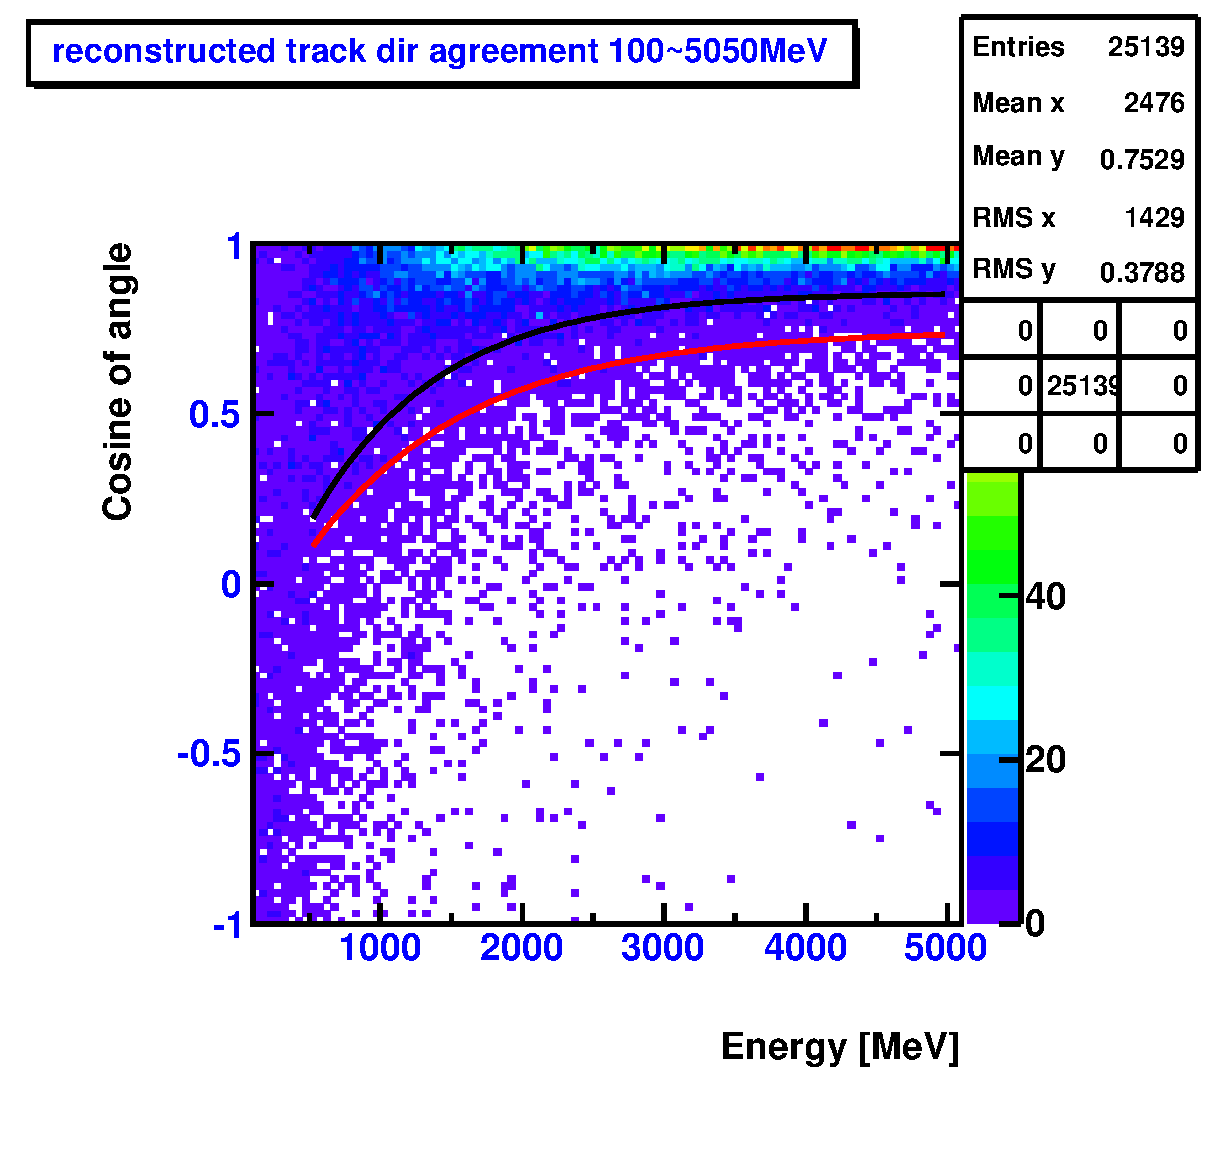
\includegraphics[width=1.0\textwidth]{analyzed_mtq_flatSpectrum_nue_C12_outerBufferFillAll_reconDirAgreementWithMtqTruthVectorVSEnergy_onlyCC_maxR600cm.eps}
	\end{columns}
	Black line: 1$\sigma$ of reconstructed angle from $\nu$ direction \\
	Red line: 1$\sigma$ of lepton angle from $\nu$ direction
\end{frame}

\begin{frame}
	\begin{itemize}
		\item Direction reconstruction is improved by fiducial volume cut on
			reconstructed vertex.
		\item What does the vertex mean for an finite size track size event?
	\end{itemize}
\end{frame}

\begin{frame}
	\frametitle{Define lepton track length as (does not include shower):}
	\begin{center}
		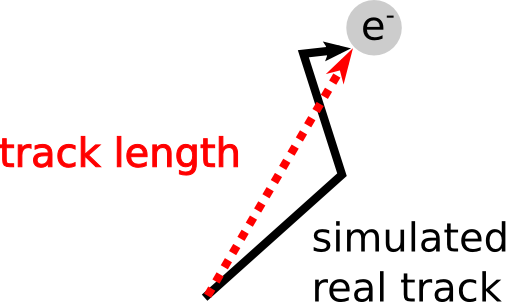
\includegraphics[height=0.2\textheight]{track_length_definition.png}
	\end{center}
	\begin{columns}[t]
		\column{0.5\textwidth}
		\ce{\nu_{e} + ^{1}H -> e^{-} + ?}
		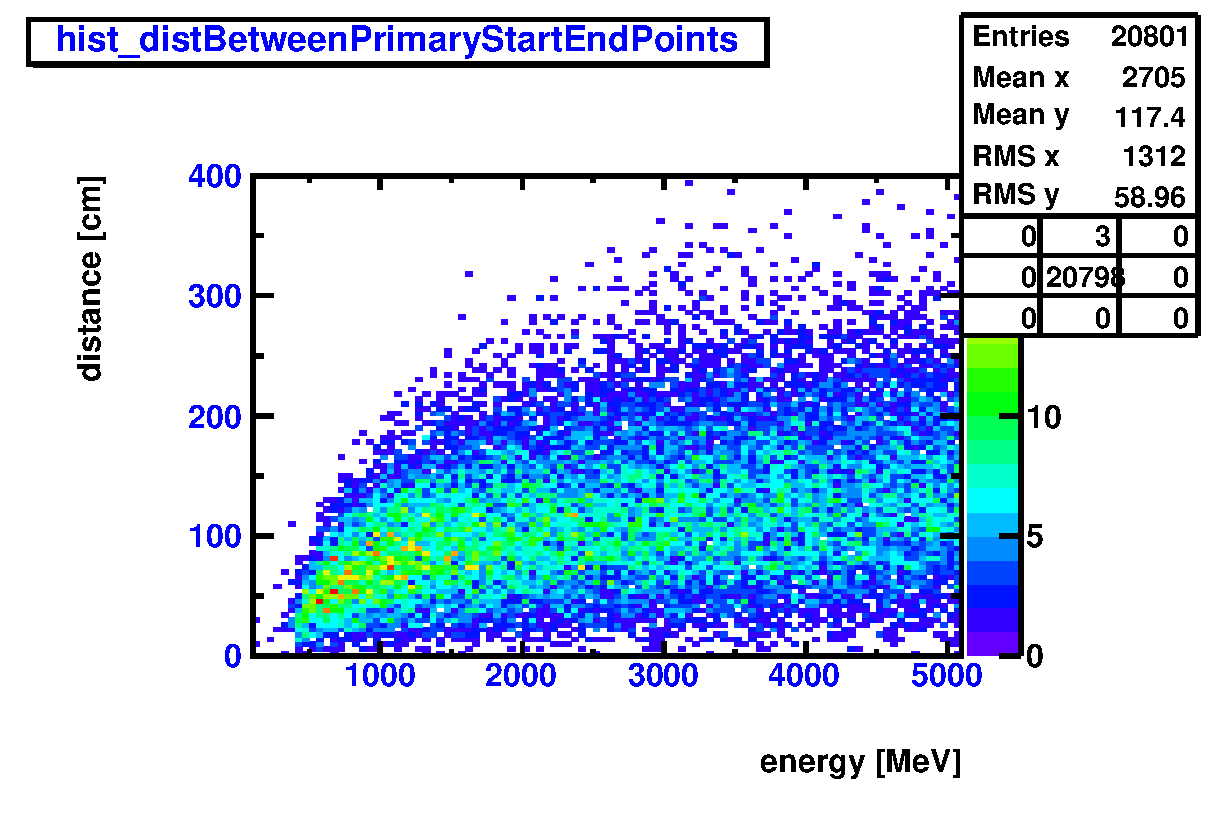
\includegraphics[width=1.0\textwidth]{nue_H1_distBetweenPrimaryStartEndPoints_onlyCC_maxR600cm.eps}
		\column{0.5\textwidth}
		\ce{\nu_{e} + ^{12}C -> e^{-} + ?}
		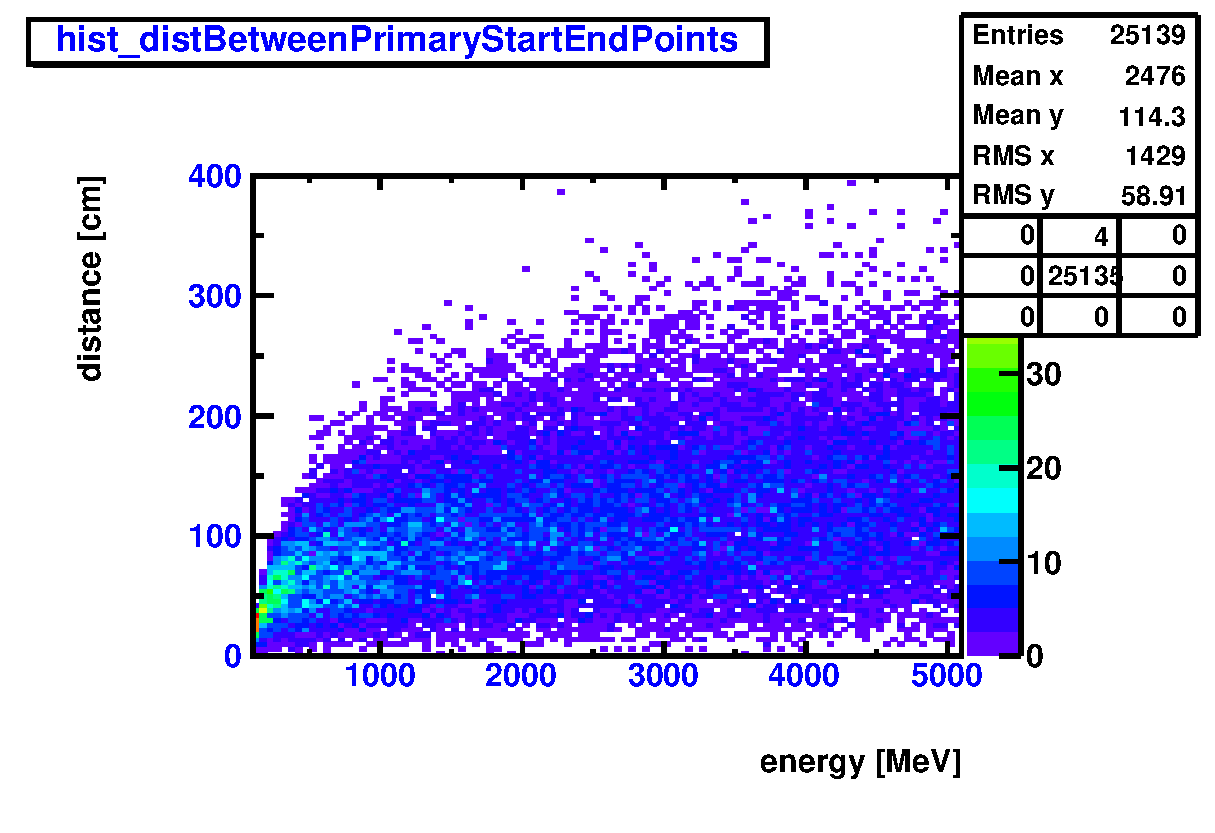
\includegraphics[width=1.0\textwidth]{nue_C12_distBetweenPrimaryStartEndPoints_onlyCC_maxR600cm.eps}
	\end{columns}
\end{frame}

\begin{frame}
	\frametitle{Perpendicular distance from reconstructed vertex to track}
	\framesubtitle{track using simulated track end points}
	\begin{center}
		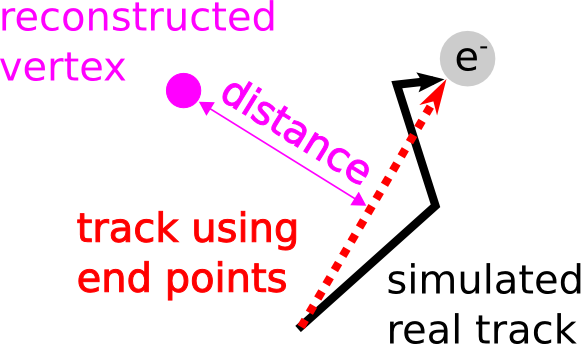
\includegraphics[height=0.2\textheight]{vertex_perpendicular_distance_from_track.png}
	\end{center}
	\begin{columns}[t]
		\column{0.5\textwidth}
		\ce{\nu_{e} + ^{1}H -> e^{-} + ?}
		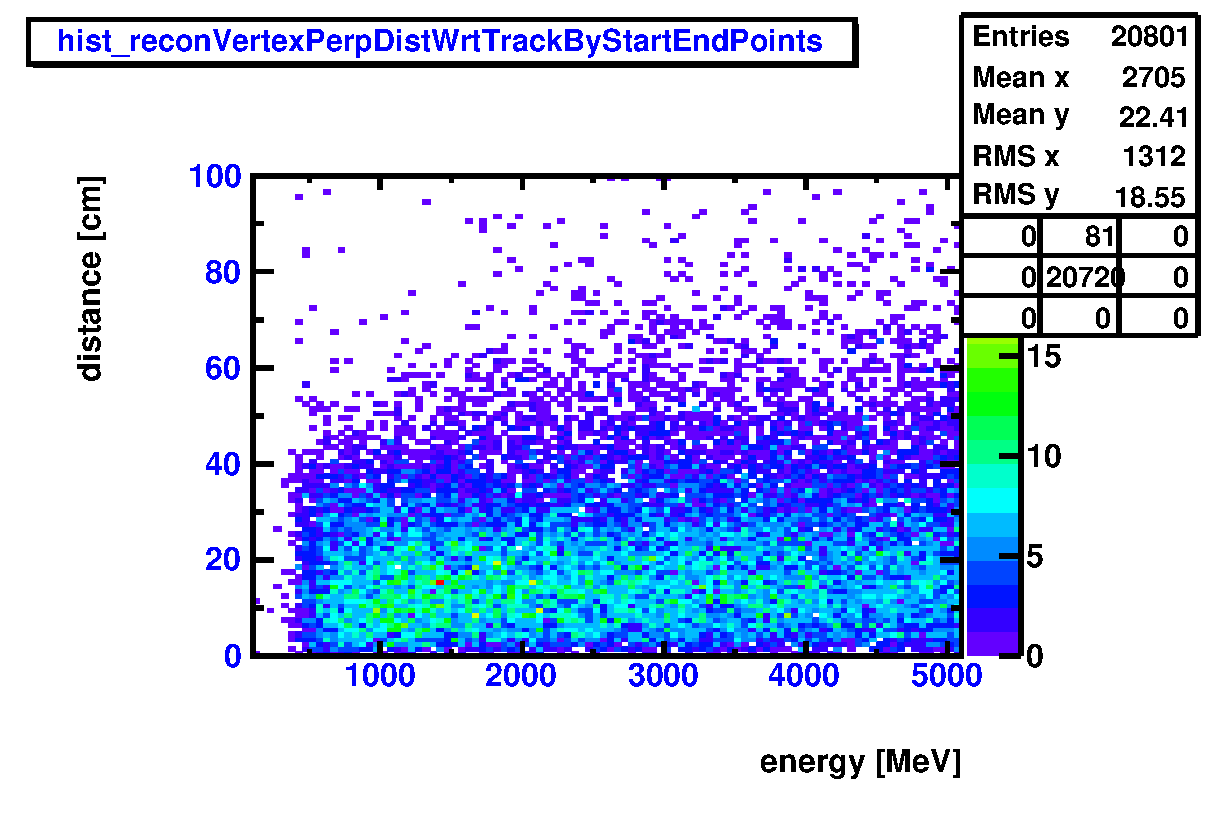
\includegraphics[width=1.0\textwidth]{nue_H1_reconVertexPerpDistWrtTrackByStartEndPoints_onlyCC_maxR600cm.eps}\\
		\column{0.5\textwidth}
		\ce{\nu_{e} + ^{12}C -> e^{-} + ?}
		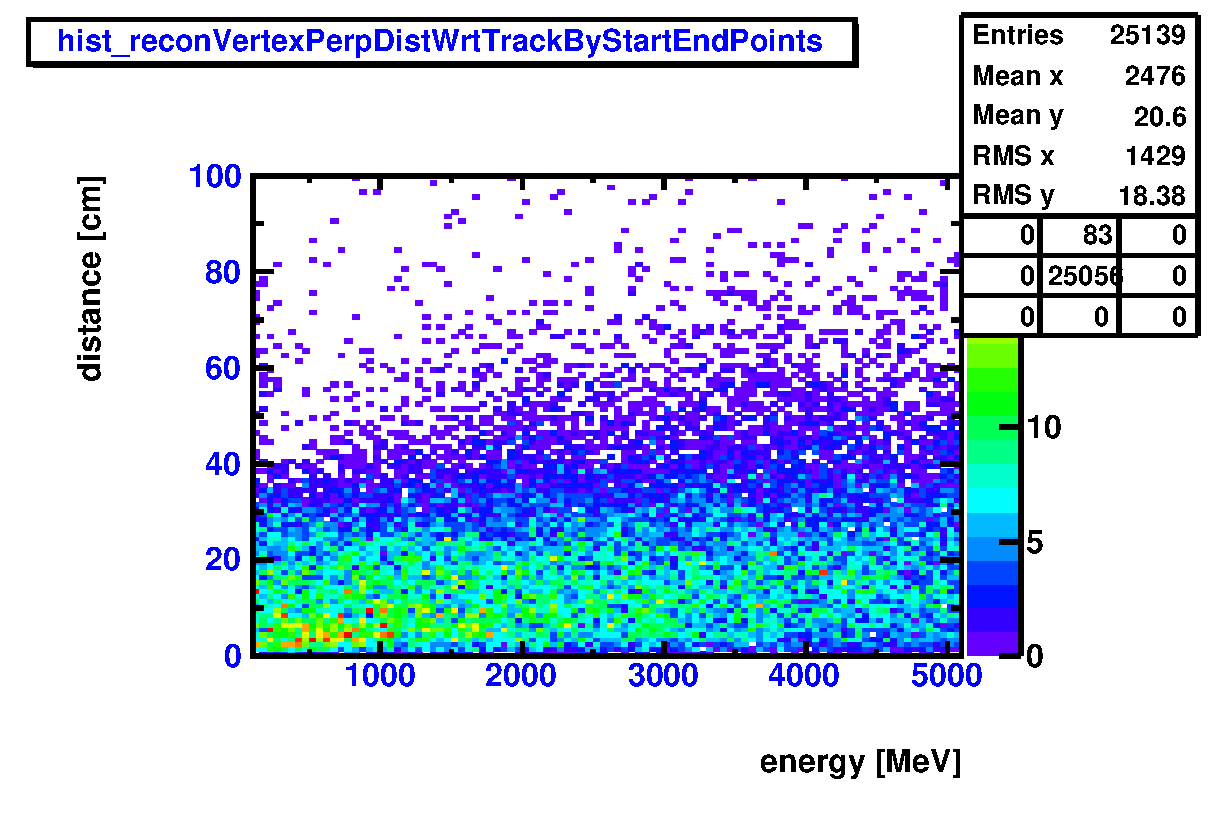
\includegraphics[width=1.0\textwidth]{nue_C12_reconVertexPerpDistWrtTrackByStartEndPoints_onlyCC_maxR600cm.eps}
	\end{columns}
\end{frame}

\begin{frame}
	\frametitle{Is the vertex reconstructed at the middle of the track?}
	\begin{center}
		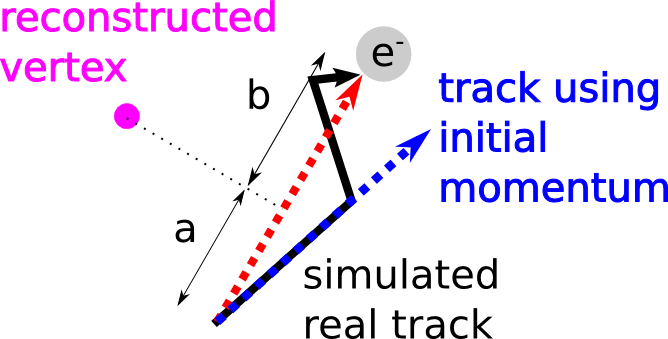
\includegraphics[height=0.4\textheight]{vertex_distance_definition.png}
	\end{center}
\end{frame}

\begin{frame}
	\frametitle{Distance of reconstructed vertex from track end points projected along tracks}
	\begin{tabular}{|C|V|V|}
		\hline
		&\ce{\nu_{e} + ^{1}H -> e^{-} + ?} &\ce{\nu_{e} + ^{12}C -> e^{-} + ?}\\
		\hline
		b &
		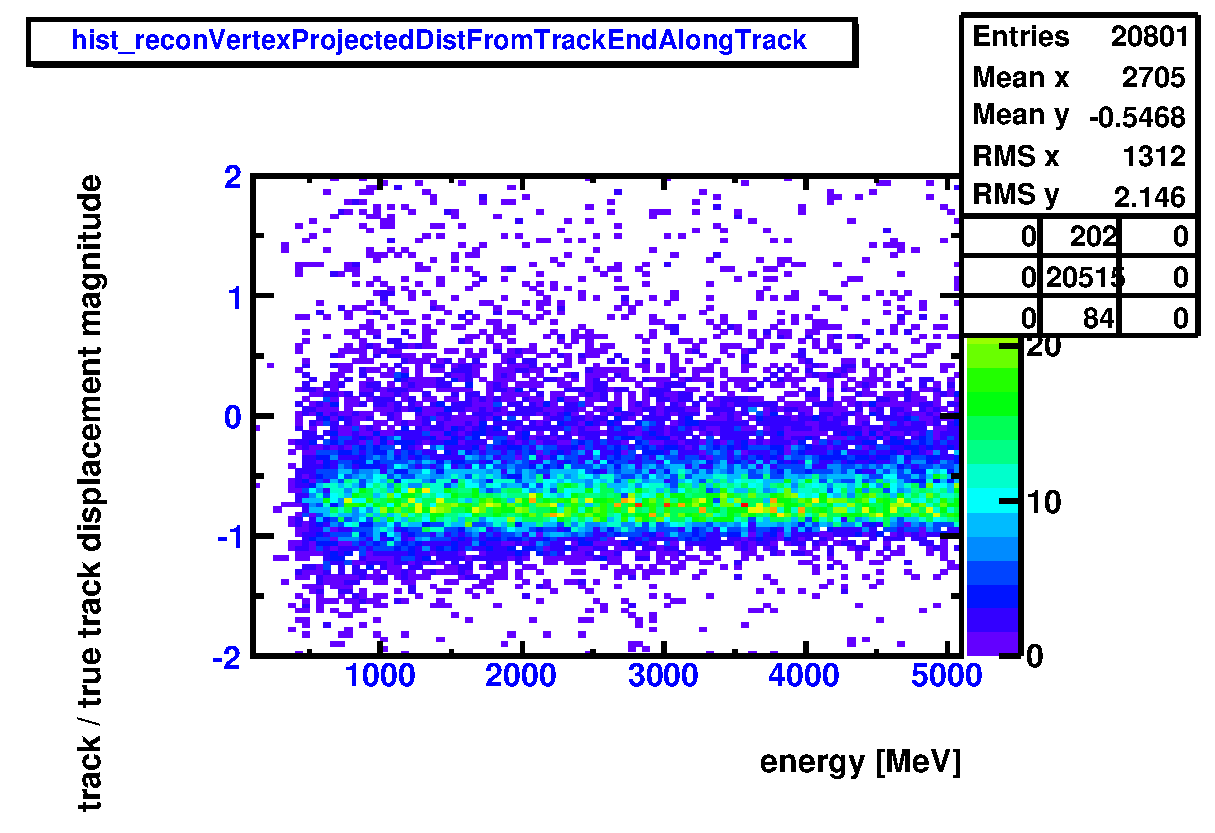
\includegraphics[width=0.45\textwidth]{nue_H1_reconVertexProjectedDistFromTrackEndAlongTrack_onlyCC_maxR600cm.eps} &
		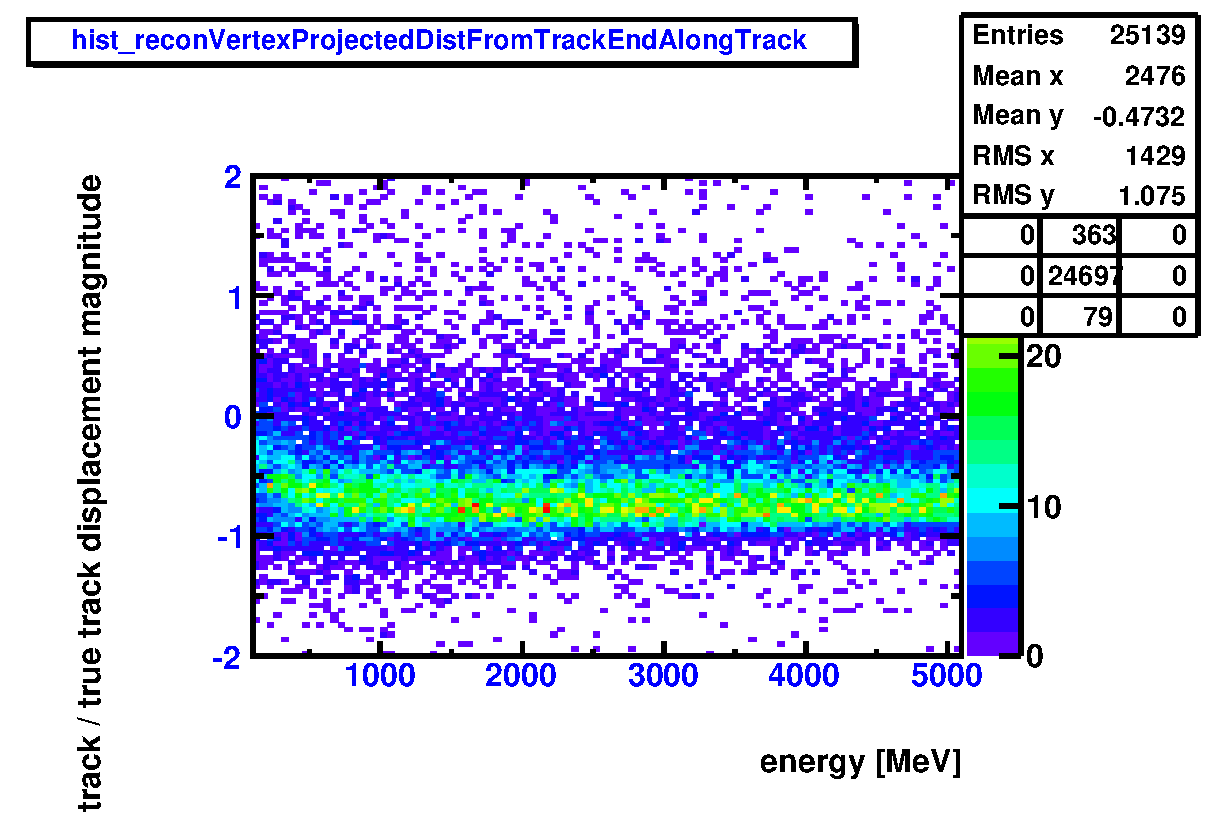
\includegraphics[width=0.45\textwidth]{nue_C12_reconVertexProjectedDistFromTrackEndAlongTrack_onlyCC_maxR600cm.eps} \\
		\hline
		a &
		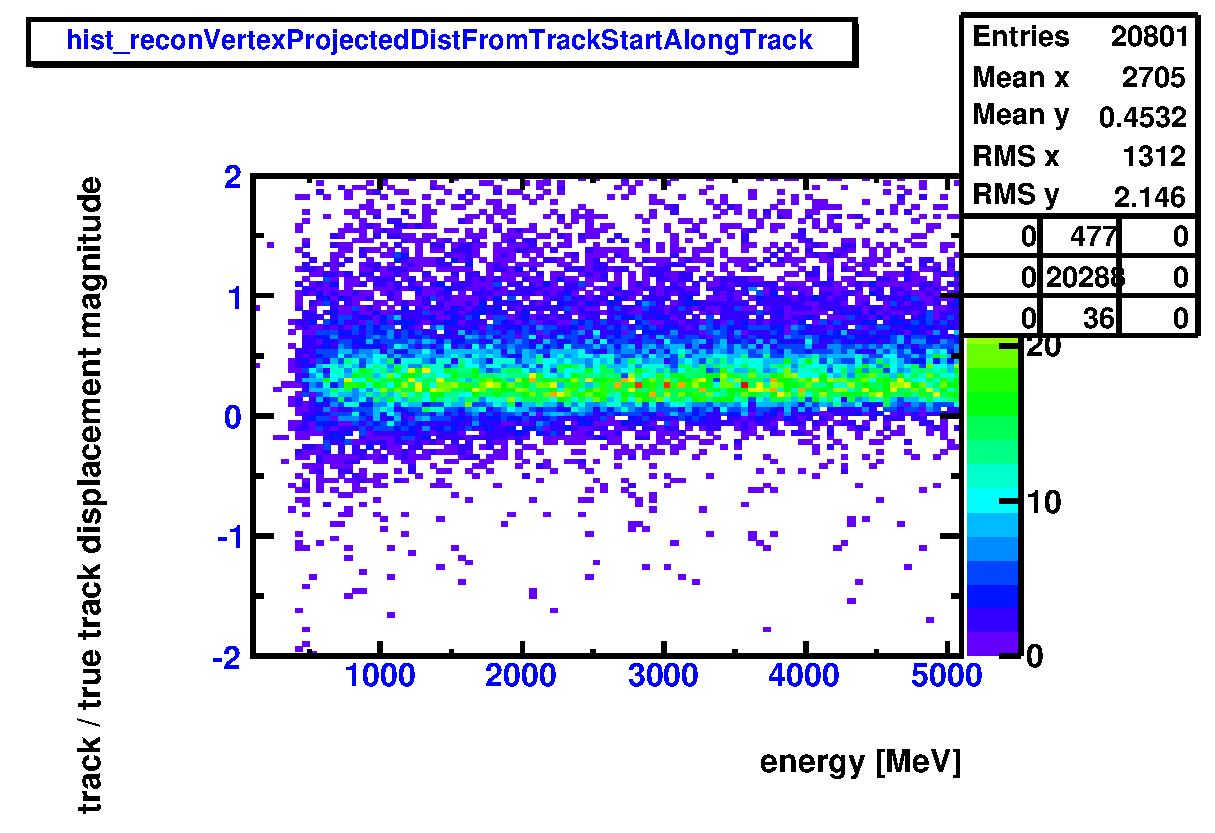
\includegraphics[width=0.45\textwidth]{nue_H1_reconVertexProjectedDistFromTrackStartAlongTrack_onlyCC_maxR600cm.eps} &
		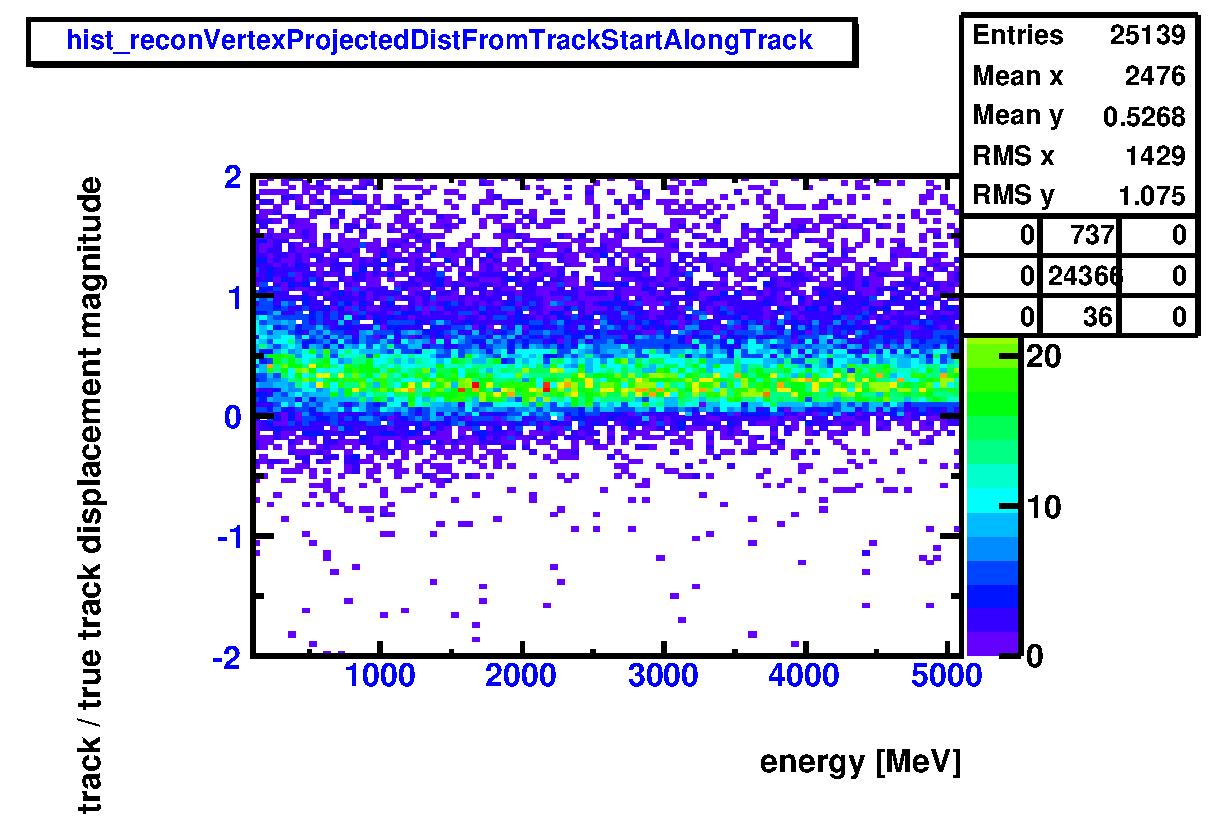
\includegraphics[width=0.45\textwidth]{nue_C12_reconVertexProjectedDistFromTrackStartAlongTrack_onlyCC_maxR600cm.eps} \\
		\hline
	\end{tabular}
\end{frame}

\begin{frame}
	\frametitle{Conclusion for reconstruction vertex}
	For $\nu_{e}$ energies \SIrange[range-phrase=--]{0.1}{5}{\giga\electronvolt}:
	\begin{itemize}
		\item Vertex is within $\sim$\SI{40}{\centi\meter} perpendicular from
			track
		\item Vertex is on average at $\sim$middle of track
		\item peak of vertex distribution is biased toward track beginning.
	\end{itemize}
\end{frame}

\begin{frame}
	\frametitle{Summary}
	\begin{itemize}
		\item High energy calibration was done using minimum ionizing muon
			events	
		\item Explored ways to cut PMT prepulsing \\
			$\rightarrow$ still work in progress (minor issue)
		\item Tested neutrino fitter with simulation for energies
			\SIrange[range-phrase=--]{0.1}{5}{\giga\electronvolt}
		\item Have minimum tools to start doing analysis for indirect Dark
			Matter search
	\end{itemize}
\end{frame}


\end{document}
